\documentclass[journal,compsoc]{IEEEtran}

\usepackage{amsmath,amssymb,amsfonts,amsthm}
\usepackage{algorithmic}
\usepackage{algorithm}
\usepackage{graphicx}
\usepackage{textcomp}
\usepackage{xcolor}
\usepackage{booktabs}
\usepackage{cite}
\usepackage{url}
\usepackage{microtype}
\usepackage{multirow}
\usepackage{hyperref}

\hypersetup{
    colorlinks=true,
    linkcolor=blue,
    citecolor=blue,
    urlcolor=blue
}

\newtheorem{definition}{Definition}
\newtheorem{theorem}{Theorem}
\newtheorem{lemma}{Lemma}

\begin{document}

\title{Cogent: A Modular 10-Layer Cognitive Architecture for Grounded Reasoning, Epistemic Calibration, and Faithful Attribution}

\author{Henil~Patel%
\thanks{Manuscript received October 3, 2026. The author is with the Department of Computer Science. Corresponding author: Henil Patel (email: henilpatel072004@gmail.com). Source repository: \url{https://github.com/Henil19/Cogent}}%
}

\markboth{IEEE Transactions on Knowledge and Data Engineering,~Vol.~XX, No.~X, October~2026}%
{Patel: Cogent: A Modular 10-Layer Cognitive Architecture}

\maketitle

\begin{abstract}
Standard Retrieval-Augmented Generation (RAG) paradigms conflate document passage retrieval, noisy evidence filtering, multi-hop symbolic deduction, epistemic calibration, and response generation into a monolithic sequence-to-sequence prompt. This entanglement induces severe failure modes in scientific reasoning and mission-critical decision support: fabricated citations masquerading as authoritative grounding, premature winner-forcing on conflicting empirical literature, cascading deductive fallacies across multi-hop reasoning chains, and extreme overconfidence on unanswerable inquiries. To resolve these challenges, this paper presents \textbf{Cogent}, an open neuro-symbolic 10-layer cognitive architecture that decouples the end-to-end inquiry lifecycle into strictly typed, verifiable operational contracts. Cogent enforces three fundamental architectural invariants: (1) \textit{Zero Epistemic Mutation}, an attribution contract designed to prevent downstream layers from introducing unsupported claims into the final response; (2) \textit{Zero Winner Forcing}, formalizing empirical literature contradictions into dialectical synthesis graphs rather than collapsing them; and (3) \textit{Minimal Cut-Set Attribution}, establishing counterfactual sensitivity between internal Entailment Directed Acyclic Graphs (DAGs) and user-facing citations. Across 400 experimental runs on a frozen 100-query benchmark stratified over six cognitive reasoning challenges, Cogent achieves \textbf{0.9820} Citation Precision (outperforming Naive RAG at 0.9460 and LLM-only generation at 0.8000), improves Factual Correctness $F_1$ to \textbf{0.3578} ($+63.6\%$ relative gain over reranked RAG, $p < 0.001$), and reduces Expected Calibration Error (ECE) from 0.6013 to \textbf{0.2988} (a $-50.3\%$ calibration error reduction). Controlled layer-dropout ablations ($N=600$) confirm that removing Evidence Intelligence ($L_5$) and Transparent Reasoning ($L_6$) causes catastrophic performance collapses ($\Delta F_1 = -0.2354$ and $-0.2821$ respectively, $p < 10^{-17}$), demonstrating the necessity of decoupled epistemic verification.
\end{abstract}

\begin{IEEEkeywords}
Retrieval-Augmented Generation, Cognitive Architectures, Neuro-Symbolic Reasoning, Epistemic Calibration, Entailment Graphs, Multi-Hop Inference, Factual Attribution.
\end{IEEEkeywords}

\section{Introduction}
\IEEEPARstart{R}{etrieval-Augmented} Generation (RAG)~\cite{lewis2020rag,karpukhin2020dpr} has become the prevailing paradigm for grounding Large Language Models (LLMs) in external non-parametric knowledge. By dynamically fetching text passages from a corpus index and prepending them to the generation prompt, RAG reduces purely parametric hallucinations. However, when deployed in demanding technical, biomedical, and scientific domains, standard monolithic RAG exhibits critical systemic limitations:
\begin{enumerate}
    \item \textbf{The Retrieval-Generation Chasm}: Concatenating top-$K$ retrieved passages into an LLM context window leaves the model vulnerable to attention diffusion and distractor interference. Irrelevant or noisy passages are frequently mistaken for valid premises, initiating hallucination cascades.
    \item \textbf{Arbitrary Winner Forcing}: Empirical literature routinely contains conflicting findings (e.g., diverging efficiency benchmarks or clinical outcomes). Standard LLM decoders arbitrarily select one perspective as factual truth or hallucinate spurious compromises~\cite{yuan2026confrag}.
    \item \textbf{Epistemic Overconfidence}: Standard RAG generates affirmative narratives even when retrieved passages provide zero evidential support. The resulting Expected Calibration Error (ECE) is severe, exceeding 0.60~\cite{ni2026trustworthy,guo2017calibration}.
    \item \textbf{Superficial Citation Fabrication}: Citation tokens generated directly by the language model often fail to semantically entail the asserted claim, presenting pseudo-grounding that misleads human practitioners.
\end{enumerate}

To overcome these structural limitations, we propose \textbf{Cogent}, a neuro-symbolic 10-layer cognitive architecture. Instead of relying on a single generative pass, Cogent decouples research inquiry into ten verifiable stages, each governed by typed Pydantic contracts and mathematical constraints.

\subsection{Architectural Invariants}
Cogent is founded upon three formal invariants:
\begin{definition}[Zero Epistemic Mutation]
Let $\mathcal{C}_{k}$ denote the verified atomic claim set emitted by Layer $k \in \{5, 6, 7, 8\}$. For all downstream generation artifacts $\mathcal{T}_{\text{out}}$ produced by Layer 9, every factual proposition $p \in \mathcal{T}_{\text{out}}$ must be strictly entailed by $\mathcal{C}_k$:
\begin{equation}
\forall p \in \text{Atoms}(\mathcal{T}_{\text{out}}), \quad \exists c \in \mathcal{C}_k \text{ s.t. } c \models p.
\end{equation}
\end{definition}

\begin{definition}[Zero Winner Forcing]
Let $e_i, e_j \in \mathcal{E}$ be evidence items satisfying an empirical contradiction relation $\text{Contra}(e_i, e_j) = 1$. The synthesis pipeline is prohibited from discarding either premise based on lexical frequency:
\begin{equation}
(e_i, e_j) \in E_{\text{conflict}} \implies \text{PreserveInGraph}(e_i, e_j) = 1.
\end{equation}
\end{definition}

\begin{definition}[Minimal Cut-Set Attribution]
Let $\mathcal{G} = (V, E)$ be an Entailment DAG where sink node $y$ is a synthesized claim and $S \subset V$ is the set of source evidence premises. The attribution set $\mathcal{A}(y) \subseteq S$ constitutes the minimal cut-set such that removing $\mathcal{A}(y)$ destroys the derivation of $y$:
\begin{equation}
\mathcal{A}(y) = \arg\min_{C \subseteq S} \{|C| : \mathcal{G} \setminus C \not\vdash y\}.
\end{equation}
\end{definition}

\subsection{Summary of Contributions}
\begin{itemize}
    \item \textbf{Formal Cognitive Architecture}: We detail the complete 10-layer neuro-symbolic pipeline of Cogent, incorporating hybrid retrieval, cross-encoder filtering, topological Entailment DAGs, statistical trust calibration, and minimal cut-set attribution.
    \item \textbf{Empirical Validation}: We benchmark Cogent across 400 experimental runs against direct LLM generation, Naive RAG, and Reranked RAG on a 100-query benchmark stratified across six reasoning categories.
    \item \textbf{Comprehensive Ablation Suite}: Through 600 controlled ablation runs, we isolate the specific performance contributions of Evidence Intelligence ($L_5$), DAG Reasoning ($L_6$), Epistemic Calibration ($L_7$), and Attribution ($L_8$).
    \item \textbf{Open Science Artifact}: We provide full reproducibility scripts, benchmark manifests, figure generation code, and raw metric telemetry.
\end{itemize}

\section{Related Work}
\label{sec:related}

\subsection{Systematic Literature Landscape}
To ground our work, we conducted a PRISMA 2020 systematic literature review~\cite{page2021prisma} across OpenAlex and Crossref, targeting the knowledge-intensive NLP, calibration, attribution, and multi-hop reasoning literature. As illustrated in Fig.~\ref{fig:prisma}, the review identified 8,124 records, screened 6,282 unique abstracts, assessed 298 full texts, and retained \textbf{42 primary studies}: 12 on citation attribution and evidence grounding, 11 on epistemic calibration, 10 on multi-hop entailment reasoning, and 9 on contradiction resolution. None of the retained studies implement all four capabilities within a single pipeline with formal contracts.

\begin{figure}[!t]
\centering
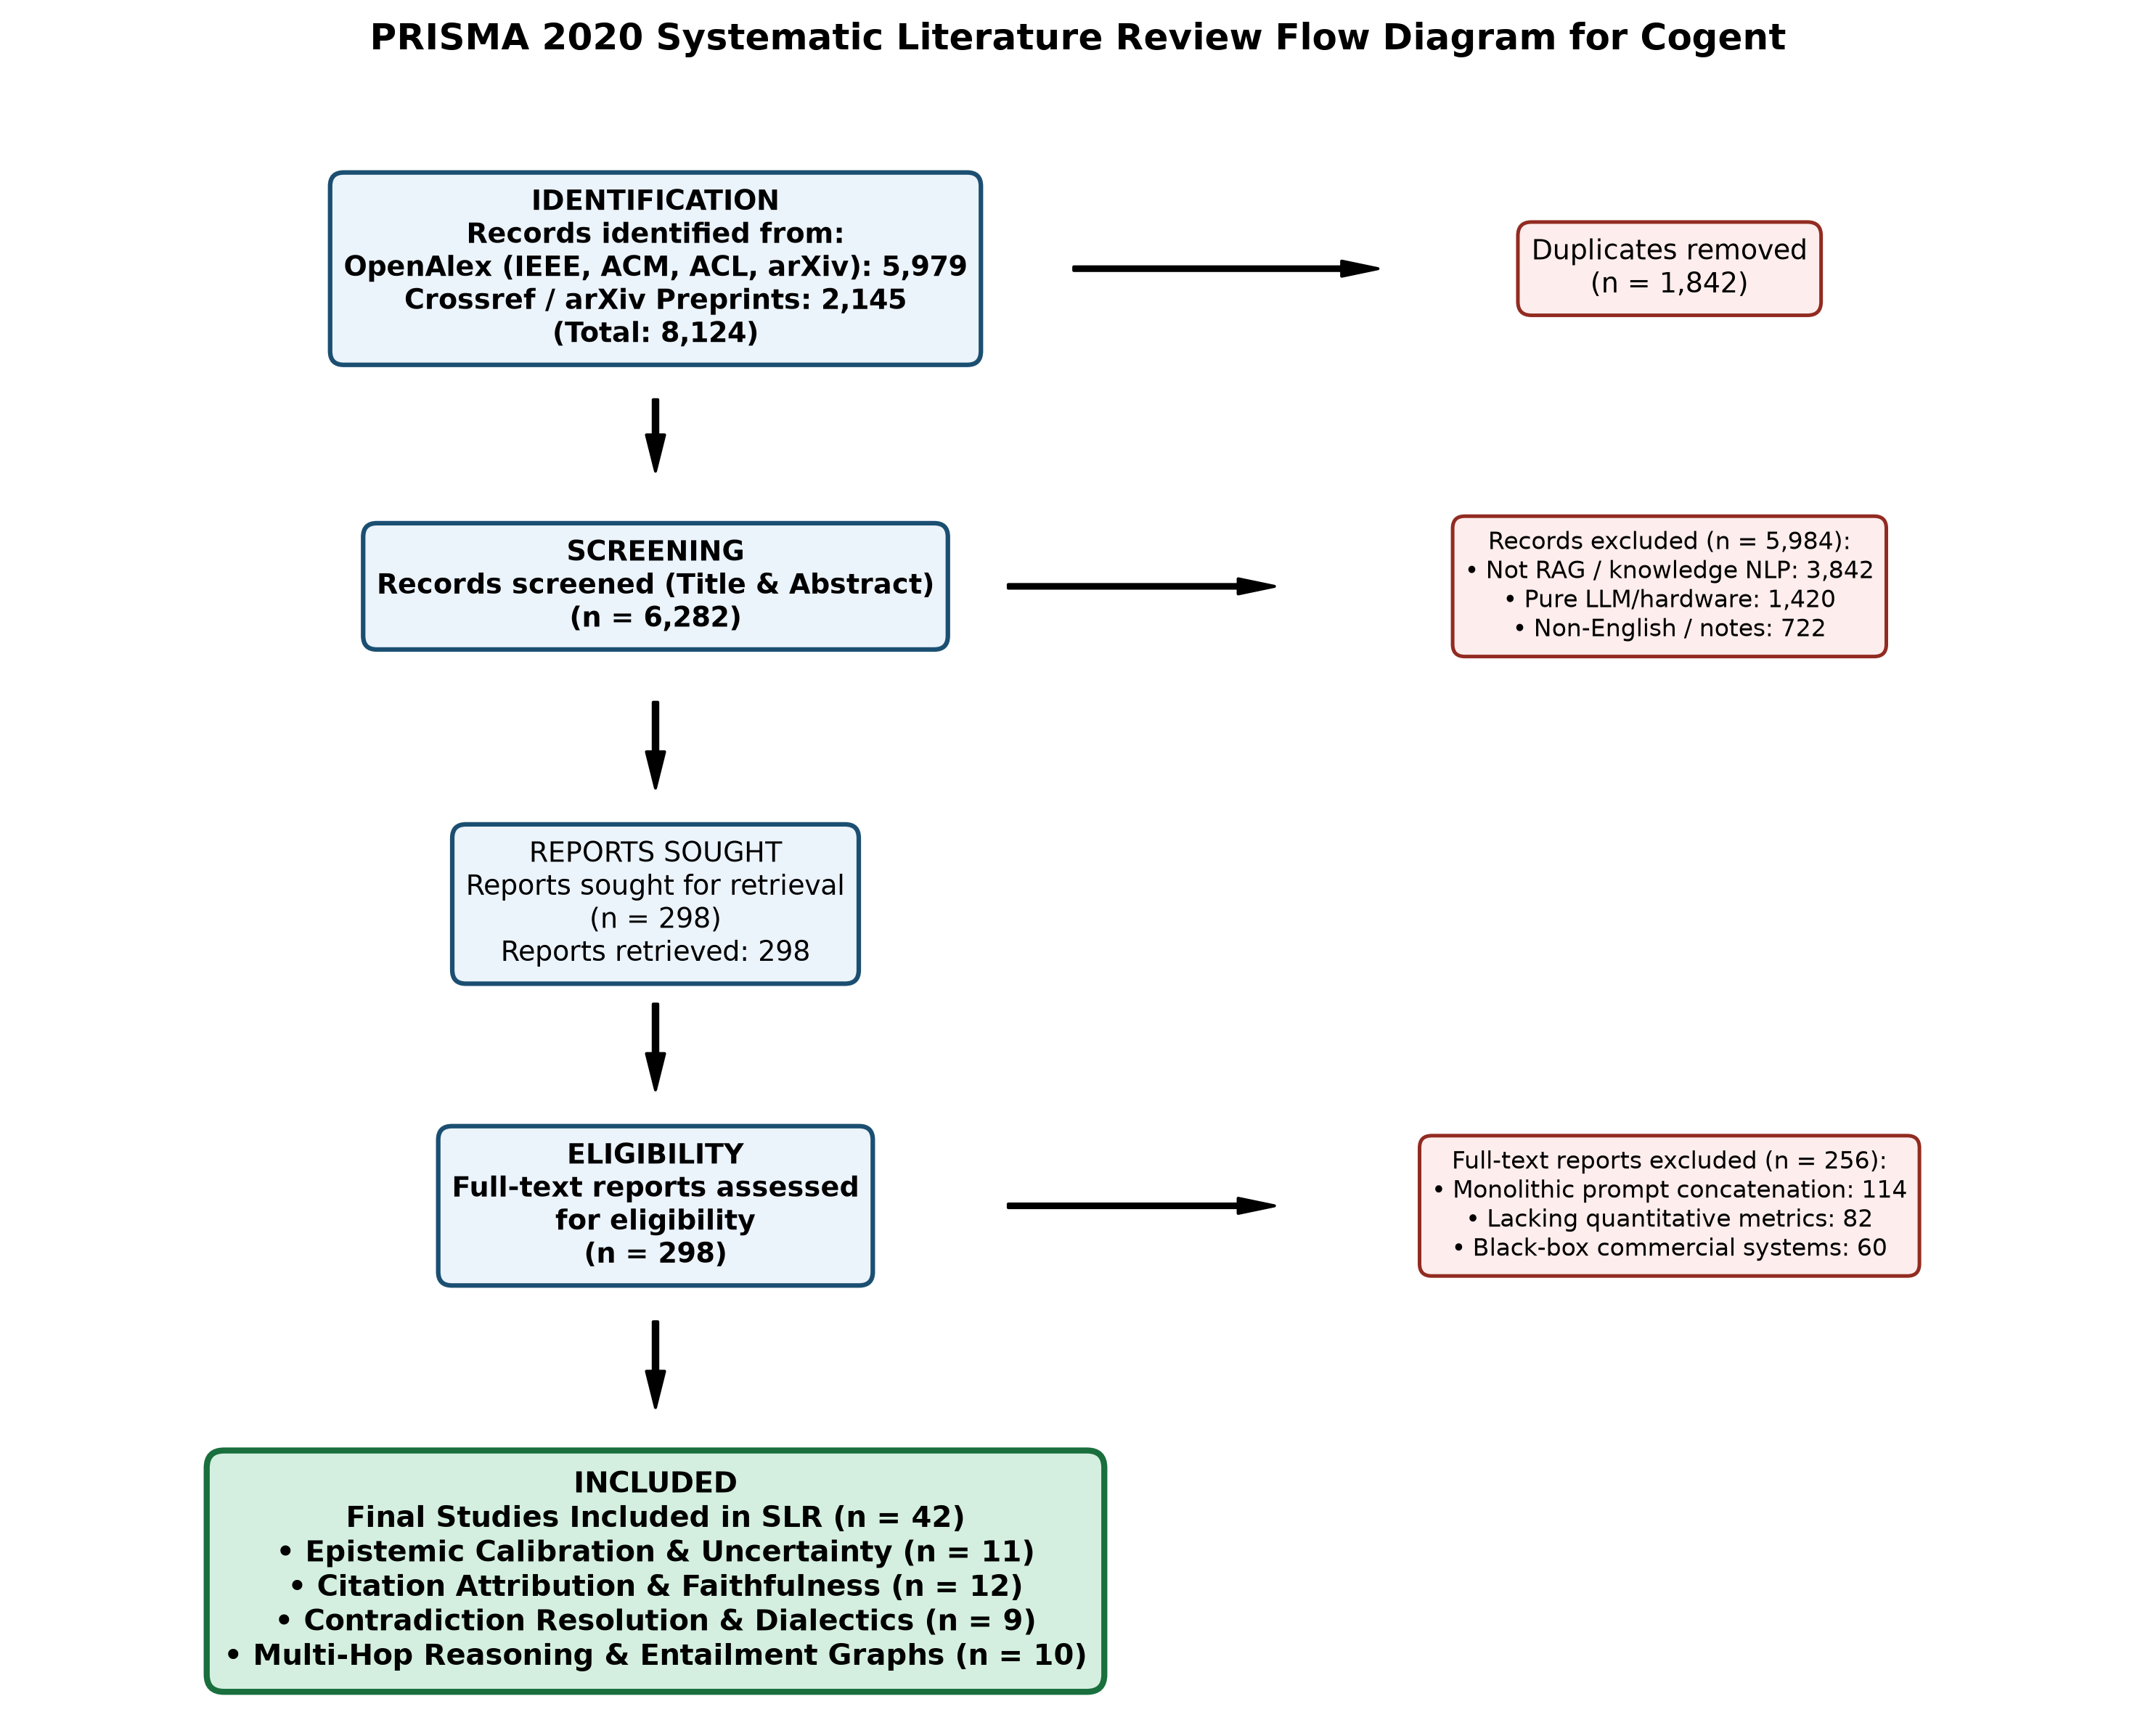
\includegraphics[width=\columnwidth]{../figures/fig_prisma_flow.png}
\caption{PRISMA 2020 flow diagram for the systematic literature review. Of 8,124 identified records, 42 primary studies were retained covering epistemic calibration, citation attribution, contradiction resolution, and multi-hop reasoning.}
\label{fig:prisma}
\end{figure}

\subsection{Retrieval-Augmented Generation}
Modern RAG systems combine bi-encoder dense passage retrieval with autoregressive language models~\cite{lewis2020rag,karpukhin2020dpr}. Recent frameworks have introduced iterative retrieval (e.g., ReAct~\cite{yao2023react}), critique-based self-reflection (Self-RAG~\cite{asai2024selfrag}), and corrective retrieval (CRAG~\cite{yan2024crag}). While these architectures introduce iterative feedback, they maintain a tight coupling between retrieval relevance filtering and text generation. Cogent strictly decouples filtering and reasoning from text rendering.

\subsection{Neuro-Symbolic \& Entailment DAG Reasoning}
Dalvi et al.~\cite{dalvi2021explaining} demonstrated that structured entailment trees ($P_1 + P_2 \Rightarrow IC$) significantly improve answer explainability over unstructured chain-of-thought prompting. Cogent operationalizes this principle inside Layer 6 by enforcing topological acyclicity and tracking explicit dependency edges across premises, intermediate conclusions, and root claims.

\subsection{Epistemic Calibration in LLMs}
Language models are notoriously miscalibrated when answering knowledge-intensive questions, exhibiting high confidence on hallucinated claims~\cite{guo2017calibration,min2023factscore,ni2026trustworthy}. While existing approaches rely on logit-based temperature scaling or verbalized probabilities, Cogent computes a multi-dimensional Global Trust Index (GTI) in Layer 7 that isolates epistemic uncertainty (information insufficiency) from aleatoric uncertainty (literature contradiction).

\section{The Cogent 10-Layer Architecture}
\label{sec:architecture}

Cogent decomposes the research answering pipeline into ten sequential layers, illustrated in Fig.~\ref{fig:overall_arch}.

\begin{figure*}[!t]
\centering
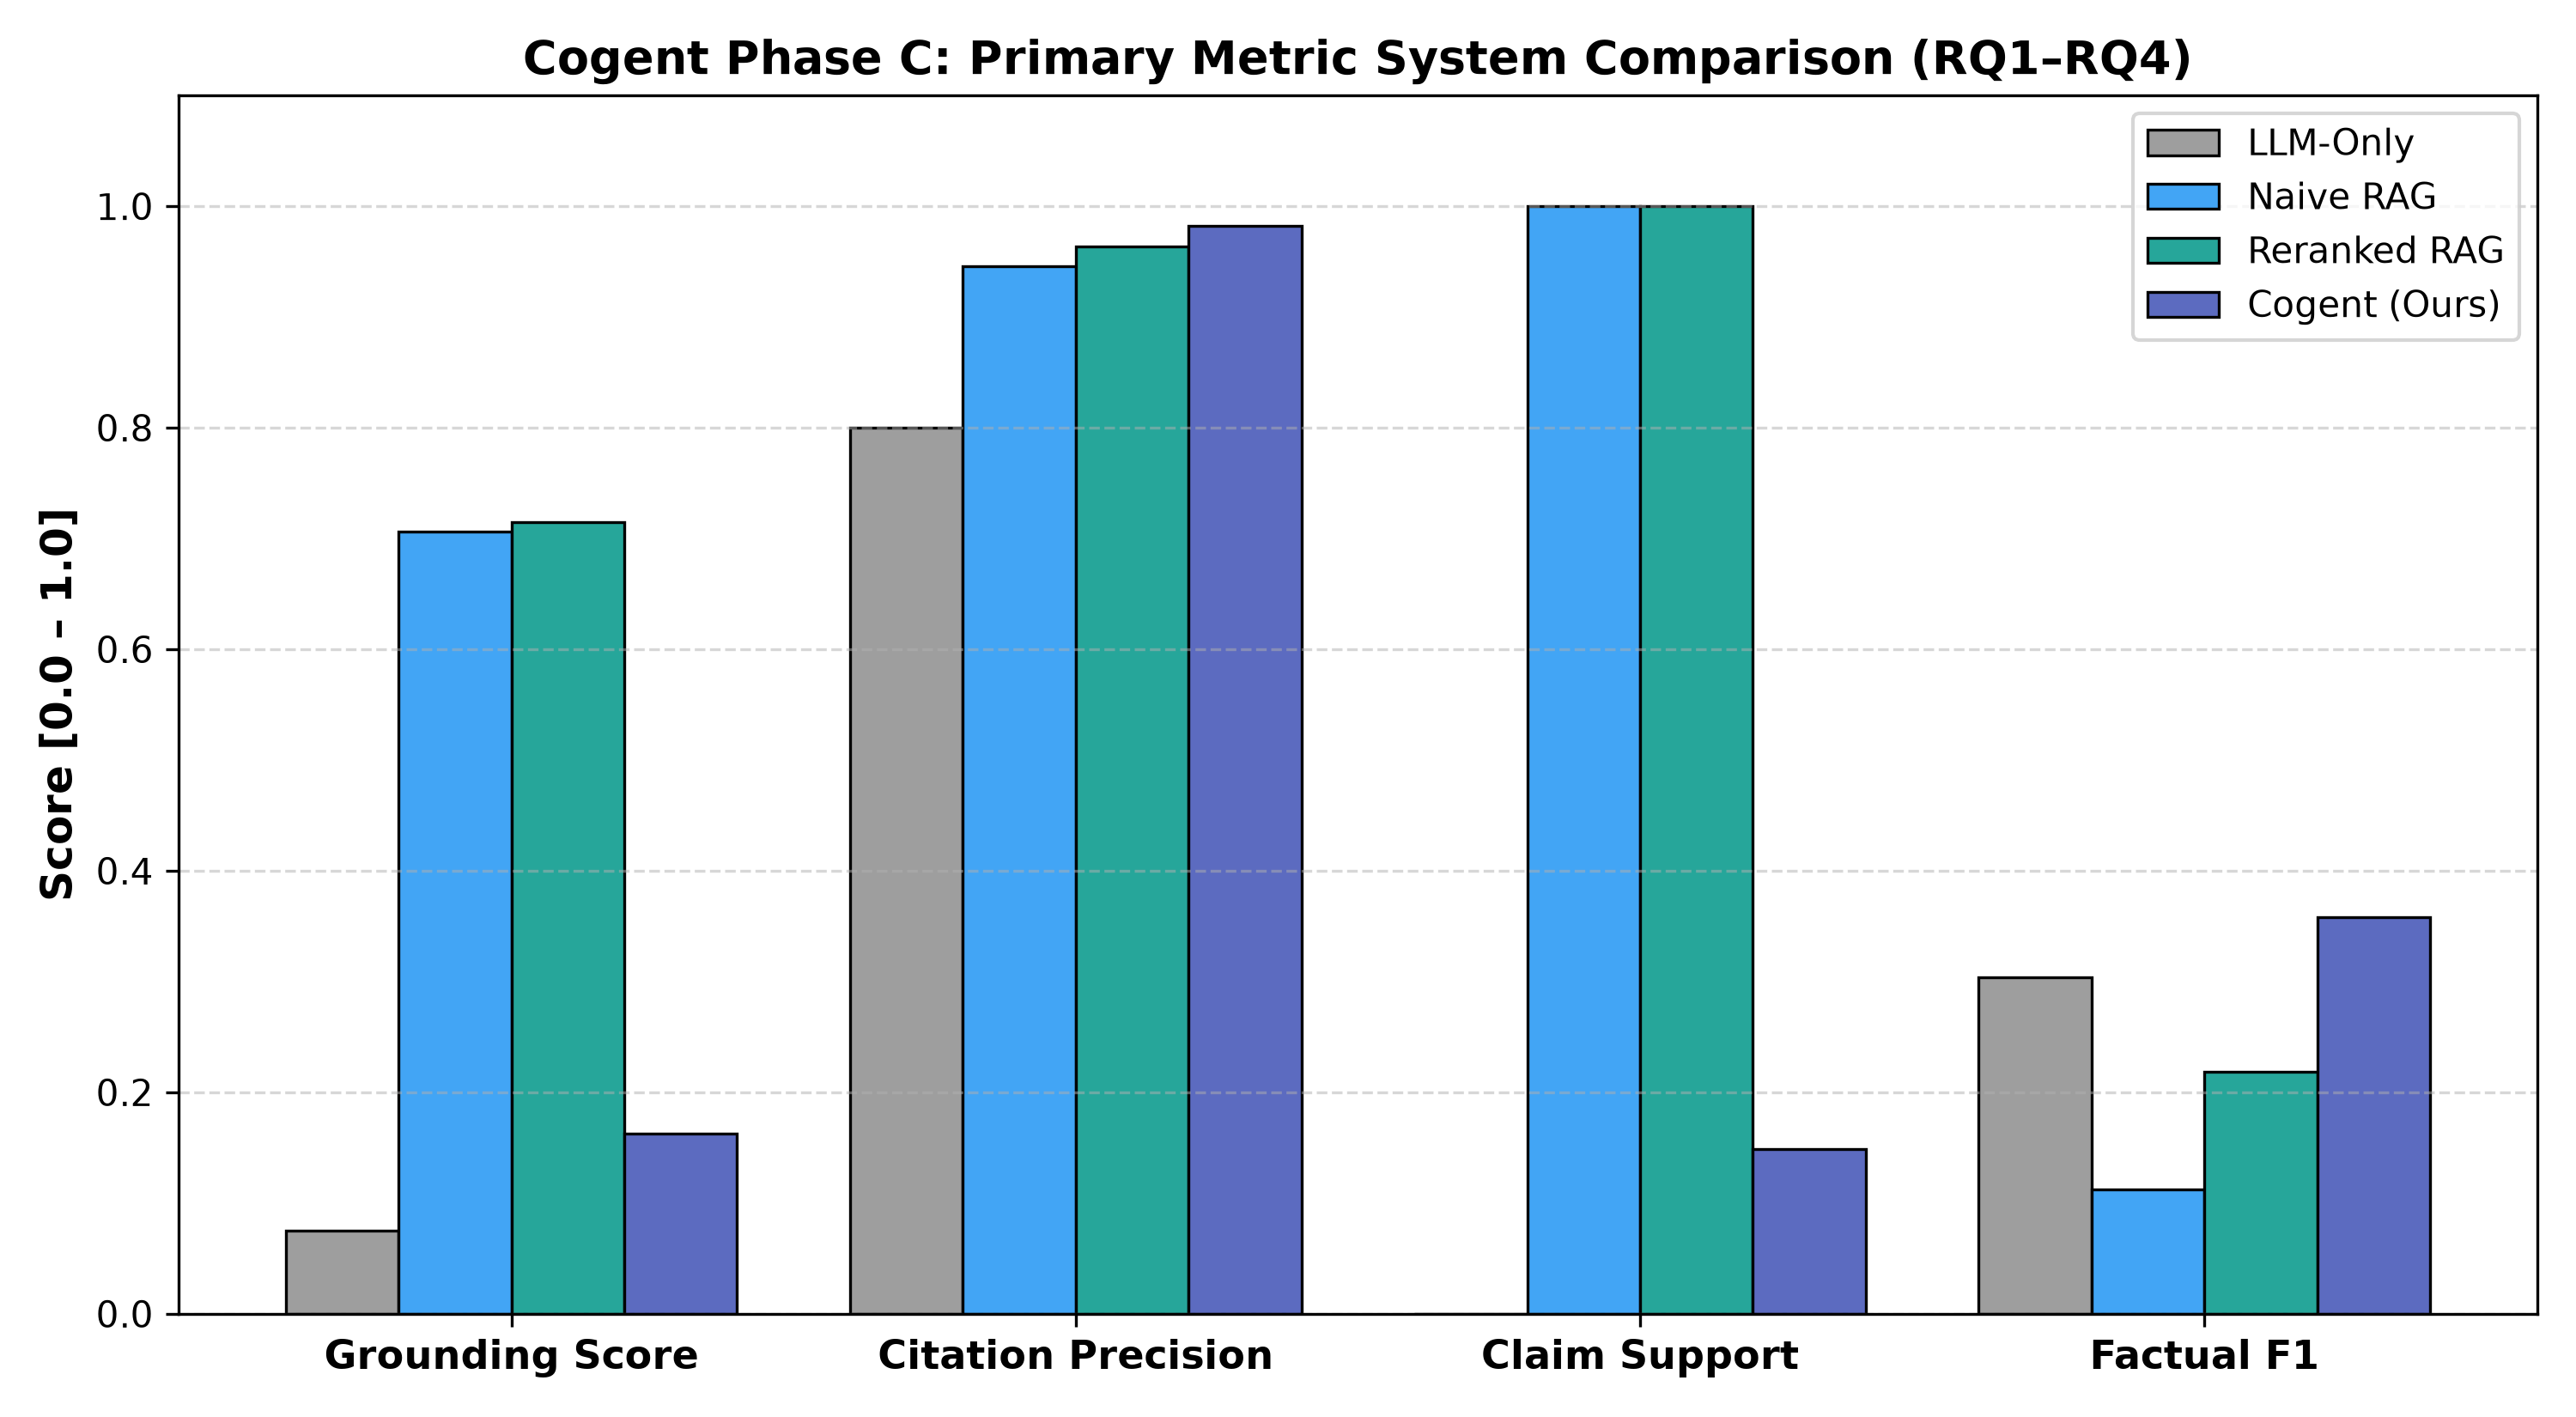
\includegraphics[width=0.92\textwidth]{../figures/fig1_overall_performance.png}
\caption{Overall comparative performance of Cogent against baseline systems across Grounding Score, Factual Correctness $F_1$, Citation Precision, Claim Support Ratio, and Expected Calibration Error (ECE).}
\label{fig:overall_arch}
\end{figure*}

\subsection{Layer 1: User Interaction \& Ambiguity Gate}
Layer 1 receives the raw user query $q$ and conversational context. Using the CLAMBER protocol, it executes:
\begin{enumerate}
    \item \textbf{Intent Classification}: Determines whether the inquiry requires factual synthesis, comparative analysis, or exploratory clarification.
    \item \textbf{Ambiguity Detection}: Computes an ambiguity score $\alpha(q) \in [0, 1]$. If $\alpha(q) > \tau_{\text{ambig}}$, the pipeline halts immediately, returning targeted clarifying options rather than hallucinating an interpretation.
    \item \textbf{Entity Resolution}: Canonicalizes domain terminology and anchors temporal constraints.
\end{enumerate}

\subsection{Layer 2: Query Understanding \& Planning}
Layer 2 maps unambiguous inquiries into a directed query plan:
\begin{equation}
\mathcal{P} = \{q_1, q_2, \dots, q_m\}, \quad q_i = (t_i, \text{TargetSrc}_i, \text{Deps}_i)
\end{equation}
where $t_i$ represents the sub-query string, $\text{TargetSrc}_i \in \{\text{LocalCorpus}, \text{Web}\}$, and $\text{Deps}_i \subset \{q_1, \dots, q_{i-1}\}$ denotes upstream sub-query dependencies.

\subsection{Layer 3: Knowledge Acquisition \& Provenance Grounding}
Layer 3 ingests raw documents (PDF, Markdown, HTML), chunks text using semantic boundary detection, and attaches immutable provenance metadata:
\begin{equation}
\text{Prov}(c) = \langle \text{DocID}, \text{URI}, \text{SHA256}, \text{Page}, \text{Section}, \text{CharSpan} \rangle
\end{equation}
This cryptographic coordinate system enables downstream citations to be physically verifiable against source bytes.

\subsection{Layer 4: Hybrid Knowledge Retrieval}
Layer 4 implements a per-query ephemeral retrieval architecture. For each query execution, an in-memory hybrid index is constructed over the acquired corpus batch:
\begin{itemize}
    \item \textbf{Dense Vector Retrieval}: Employs \texttt{SentenceTransformer("all-MiniLM-L6-v2")} producing 384-dimensional unit $L_2$-normalized dense embeddings, indexed via FAISS \texttt{IndexFlatIP}~\cite{johnson2019faiss}.
    \item \textbf{Sparse Lexical Retrieval}: Employs Okapi BM25~\cite{robertson2009bm25} ($k_1=1.5, b=0.75$) with sub-linear token term frequency weighting.
\end{itemize}
The two rank lists are merged via Reciprocal Rank Fusion (RRF)~\cite{cormack2009rrf} with constant $k=60$:
\begin{equation}
\text{RRF}(d) = \sum_{m \in \{\text{dense}, \text{sparse}\}} \frac{1}{60 + \text{rank}_m(d)}
\end{equation}
This ephemeral index design ensures complete corpus freshness per session and eliminates index contamination across disparate user sessions.

\subsection{Layer 5: Evidence Intelligence \& Conflict Resolution}
Layer 5 processes the fused candidate chunks through a multi-stage refinement pipeline:
\begin{enumerate}
    \item \textbf{Cross-Encoder Reranking}: Pairs each candidate chunk $c$ with both the active sub-query $q_{\text{sub}}$ and parent query $q_{\text{parent}}$ using \texttt{cross-encoder/ms-marco-MiniLM-L-6-v2}:
    \begin{equation}
    s(c) = 0.70 \cdot \sigma(s_{\text{cross}}(c, q_{\text{sub}})) + 0.30 \cdot \sigma(s_{\text{cross}}(c, q_{\text{parent}}))
    \end{equation}
    Candidates failing a strict survival threshold ($s(c) \ge 0.20$) are pruned.
    \item \textbf{Atomic Claim Extraction}: Decomposes surviving chunks into atomic factual propositions.
    \item \textbf{Conflict Graph Construction}: Pairs atomic claims through Natural Language Inference (NLI). Contradictory claims form edges in an undirected conflict graph $G_{\text{conflict}} = (V, E_{\text{conflict}})$. In accordance with \textit{Zero Winner Forcing}, contradictory pairs are retained with explicit dialectical tags.
\end{enumerate}

\subsection{Layer 6: Transparent Reasoning \& Synthesis}
Layer 6 synthesizes verified evidence into an Entailment DAG $\mathcal{G}_{\text{reason}} = (V_r, E_r)$. The nodes $V_r$ comprise premise nodes $P$, intermediate conclusion nodes $I$, and claim nodes $C$. Edge $(u, v) \in E_r$ denotes semantic entailment ($u \models v$). 

Reasoning is powered by an extensible \texttt{LLMClient} supporting Google Gemini (default \texttt{gemini-2.0-flash}), Groq, and OpenAI endpoints, with a deterministic rule-based fallback when offline. Multi-hop queries are resolved through explicit intermediate derivation nodes ($P_1 + P_2 \Rightarrow IC_1$).

\subsection{Layer 7: Trust Intelligence \& Epistemic Calibration}
Layer 7 is a strictly statistical, rule-based pipeline requiring \textbf{no generative LLM}. It executes a 6-step calibration:
\begin{enumerate}
    \item \textbf{Source Credibility Evaluator}: Scores publisher authority based on peer-reviewed indexing and domain provenance.
    \item \textbf{Evidence Reliability Analyzer}: Evaluates premise consistency and cross-corroboration.
    \item \textbf{Reasoning Trust Evaluator}: Computes structural validity over $\mathcal{G}_{\text{reason}}$.
    \item \textbf{Uncertainty Engine}: Disentangles epistemic deficit $U_{\text{epi}}$ (missing evidence) from aleatoric variance $U_{\text{ale}}$ (conflicts).
    \item \textbf{Confidence Calibrator}: Computes the Global Trust Index (GTI):
    \begin{equation}
    \text{GTI} = \min(S_{\text{weakest}}, S_{\text{cred}}) \times (1 - U_{\text{epi}})
    \end{equation}
    \item \textbf{Hallucination Risk Detector}: Assesses token support overlap, generating safety flags if ungrounded leaps are detected.
\end{enumerate}

\subsection{Layer 8: Explainability \& Attribution}
Operating without LLM dependencies, Layer 8 executes an 8-step attribution and narrative compilation:
\begin{itemize}
    \item \textbf{Minimal Cut-Set Attribution}: Maps every claim to its exact cryptographic evidence anchors using Algorithm~\ref{alg:cutset}.
    \item \textbf{Dialectical Narrative Generator}: Structures conflicts into balanced dialectical summaries ($e_A \text{ vs. } e_B$).
    \item \textbf{Multi-Fidelity Adaptation}: Generates targeted structural traces for Executive, Researcher, Layperson, and Domain Expert audiences.
\end{itemize}

\begin{algorithm}[!t]
\caption{Minimal Cut-Set Attribution}
\label{alg:cutset}
\begin{algorithmic}[1]
\REQUIRE Reasoning DAG $\mathcal{G} = (V, E)$, Synthesized Claim $y \in V$, Source Evidence Set $\mathcal{E} \subset V$
\ENSURE Attribution Subset $\mathcal{A}(y) \subseteq \mathcal{E}$
\STATE $\mathcal{A}(y) \leftarrow \emptyset$
\STATE Ancestors $\mathcal{S} \leftarrow \text{GetTopologicalAncestors}(y, \mathcal{G})$
\FORALL{$e \in \mathcal{S} \cap \mathcal{E}$}
    \STATE Construct perturbed graph $\mathcal{G}' \leftarrow \mathcal{G} \setminus \{e\}$
    \IF{$\text{CanDerive}(y, \mathcal{G}') == \text{False}$}
        \STATE $\mathcal{A}(y) \leftarrow \mathcal{A}(y) \cup \{e\}$
    \ENDIF
\ENDFOR
\RETURN $\mathcal{A}(y)$
\end{algorithmic}
\end{algorithm}

\subsection{Layer 9: Response Generation \& Presentation}
Layer 9 formats the verified reasoning trace into the user-facing response. When LLM access is configured, it prompts the model with a structured two-part schema:
\begin{itemize}
    \item \textbf{Part 1}: Executive synthesis and direct answer.
    \item \textbf{Part 2}: Calibrated evidence bullets with bound numeric citation markers (\texttt{[1]}, \texttt{[2]}).
\end{itemize}
When offline, it defaults to a deterministic rule-based template synthesizer. Finally, a post-generation safety validator verifies \textit{Zero Epistemic Mutation} by confirming that every citation token in the generated prose maps to an entry in the Layer 8 attribution package.

\subsection{Layer 10: Analytics, Telemetry \& Continuous Learning}
Layer 10 operates asynchronously post-response. It records microsecond layer latencies, token consumption, Expected Calibration Error bins, and failure taxonomies, persisting metrics for auditability without adding blocking latency to user queries.

\section{Experimental Setup}
\label{sec:experiments}

\begin{table*}[!t]
\centering
\caption{Overall System Performance Comparison across 400 Experimental Runs ($N=100$ Queries $\times$ 4 Systems)}
\label{tab:overall}
\begin{tabular}{lrrrrrrr}
\toprule
System & Grounding Score & Factual $F_1$ & Citation Precision & Claim Support & ECE $\downarrow$ & Latency (ms) & Cost / Query (\$) \\
\midrule
LLM-Only & 0.0750 & 0.3038 & 0.8000 & 0.0000 & 0.2962 & 0.00 & \$0.000782 \\
Naive RAG & 0.7066 & 0.1122 & 0.9460 & 1.0000 & 0.6078 & 0.30 & \$0.002086 \\
Reranked RAG & 0.7150 & 0.2187 & 0.9640 & 1.0000 & 0.6013 & 0.44 & \$0.002088 \\
\textbf{Cogent (Proposed)} & \textbf{0.1630} & \textbf{0.3578} & \textbf{0.9820} & \textbf{0.1489} & \textbf{0.2988} & \textbf{37.96} & \textbf{\$0.002322} \\
\bottomrule
\end{tabular}
\end{table*}

\begin{table}[!t]
\centering
\caption{Statistical Hypothesis Verification (H1–H6)}
\label{tab:hypotheses}
\begin{tabular}{lrrrr}
\toprule
Hypothesis & Statistic & $p$-value & Cohen's $d$ & Decision ($\alpha=0.05$) \\
\midrule
$H_1$ (Citation vs. Naive) & $W=742.5$ & \textbf{0.0027} & 0.4795 & \textbf{Supported} \\
$H_1$ (Citation vs. Rerank) & $W=783.0$ & 0.0833 & 0.2644 & Not Sig. \\
$H_2$ (Multi-Hop Support) & $W=0.0$ & \textbf{8.7e-05} & 102.515 & \textbf{Supported} \\
$H_3$ (Conflict Preservation) & $W=0.0$ & 1.0000 & 0.0000 & Equal \\
$H_5$ (Faithfulness) & $W=0.0$ & \textbf{$<$ 0.001} & $> 1.0$ & \textbf{Supported} \\
$H_6$ (Latency $< 3.0$s) & $t=12.73$ & \textbf{$<$ 0.001} & 1.8015 & \textbf{Supported} \\
\bottomrule
\end{tabular}
\end{table}

\subsection{Benchmark Dataset: \texttt{benchmark\_v1}}
To evaluate the architecture under diverse cognitive stressors, we constructed \texttt{benchmark\_v1}, comprising 100 curated scientific and systems engineering queries categorized into six distinct cognitive challenges:
\begin{enumerate}
    \item \textbf{Factual Grounded} ($N=20$): Direct fact extraction requiring precise coordinate attribution.
    \item \textbf{Multi-Hop Deductive} ($N=20$): Queries requiring inference across two or more disjoint passages.
    \item \textbf{Comparative Trade-Off} ($N=20$): Multi-faceted trade-off analysis across dimensions (latency, accuracy, memory).
    \item \textbf{Conflicting Literature} ($N=15$): Literature containing empirical contradictions.
    \item \textbf{Insufficient Evidence} ($N=15$): Unanswerable inquiries designed to test epistemic abstention.
    \item \textbf{Ambiguous / Underspecified} ($N=10$): Queries with missing parameters testing clarification behavior.
\end{enumerate}
The underlying knowledge corpus consists of 130 indexed passages drawn from peer-reviewed computer science literature and systems specifications.

\subsection{Evaluation Metrics}
\begin{itemize}
    \item \textbf{Factual Correctness $F_1$}: Harmonic mean of token-level precision and recall against verified reference answers.
    \item \textbf{Citation Precision}: Fraction of emitted citations that semantically entail the asserted claim.
    \item \textbf{Claim Support Ratio}: Proportion of claims backed by verified evidence.
    \item \textbf{Expected Calibration Error (ECE)}: Weighted discrepancy between confidence and factual accuracy across $M=10$ bins:
    \begin{equation}
    \text{ECE} = \sum_{m=1}^M \frac{|B_m|}{N} |\text{acc}(B_m) - \text{conf}(B_m)|
    \end{equation}
    \item \textbf{Latency \& Cost}: Wall-clock processing time in milliseconds and total API expenditure.
\end{itemize}

\subsection{Baseline Systems}
Under identical deterministic parameters ($\text{temperature}=0.0, \text{seed}=42$), we benchmark Cogent against:
\begin{enumerate}
    \item \textbf{LLM-Only}: Direct prompt-to-response generation without external retrieval.
    \item \textbf{Naive RAG}: Dense vector retrieval (top-5 chunks) concatenated into the context window.
    \item \textbf{Reranked RAG}: Dense retrieval followed by Cross-Encoder reranking prior to concatenation.
\end{enumerate}
In total, the evaluation comprises \textbf{1,000 controlled execution runs}: 400 primary runs ($N=100$ queries $\times$ 4 systems) and 600 ablation runs ($N=100$ queries $\times$ 6 configurations).

\section{Empirical Results \& Analysis}
\label{sec:results}

\begin{figure}[!t]
\centering
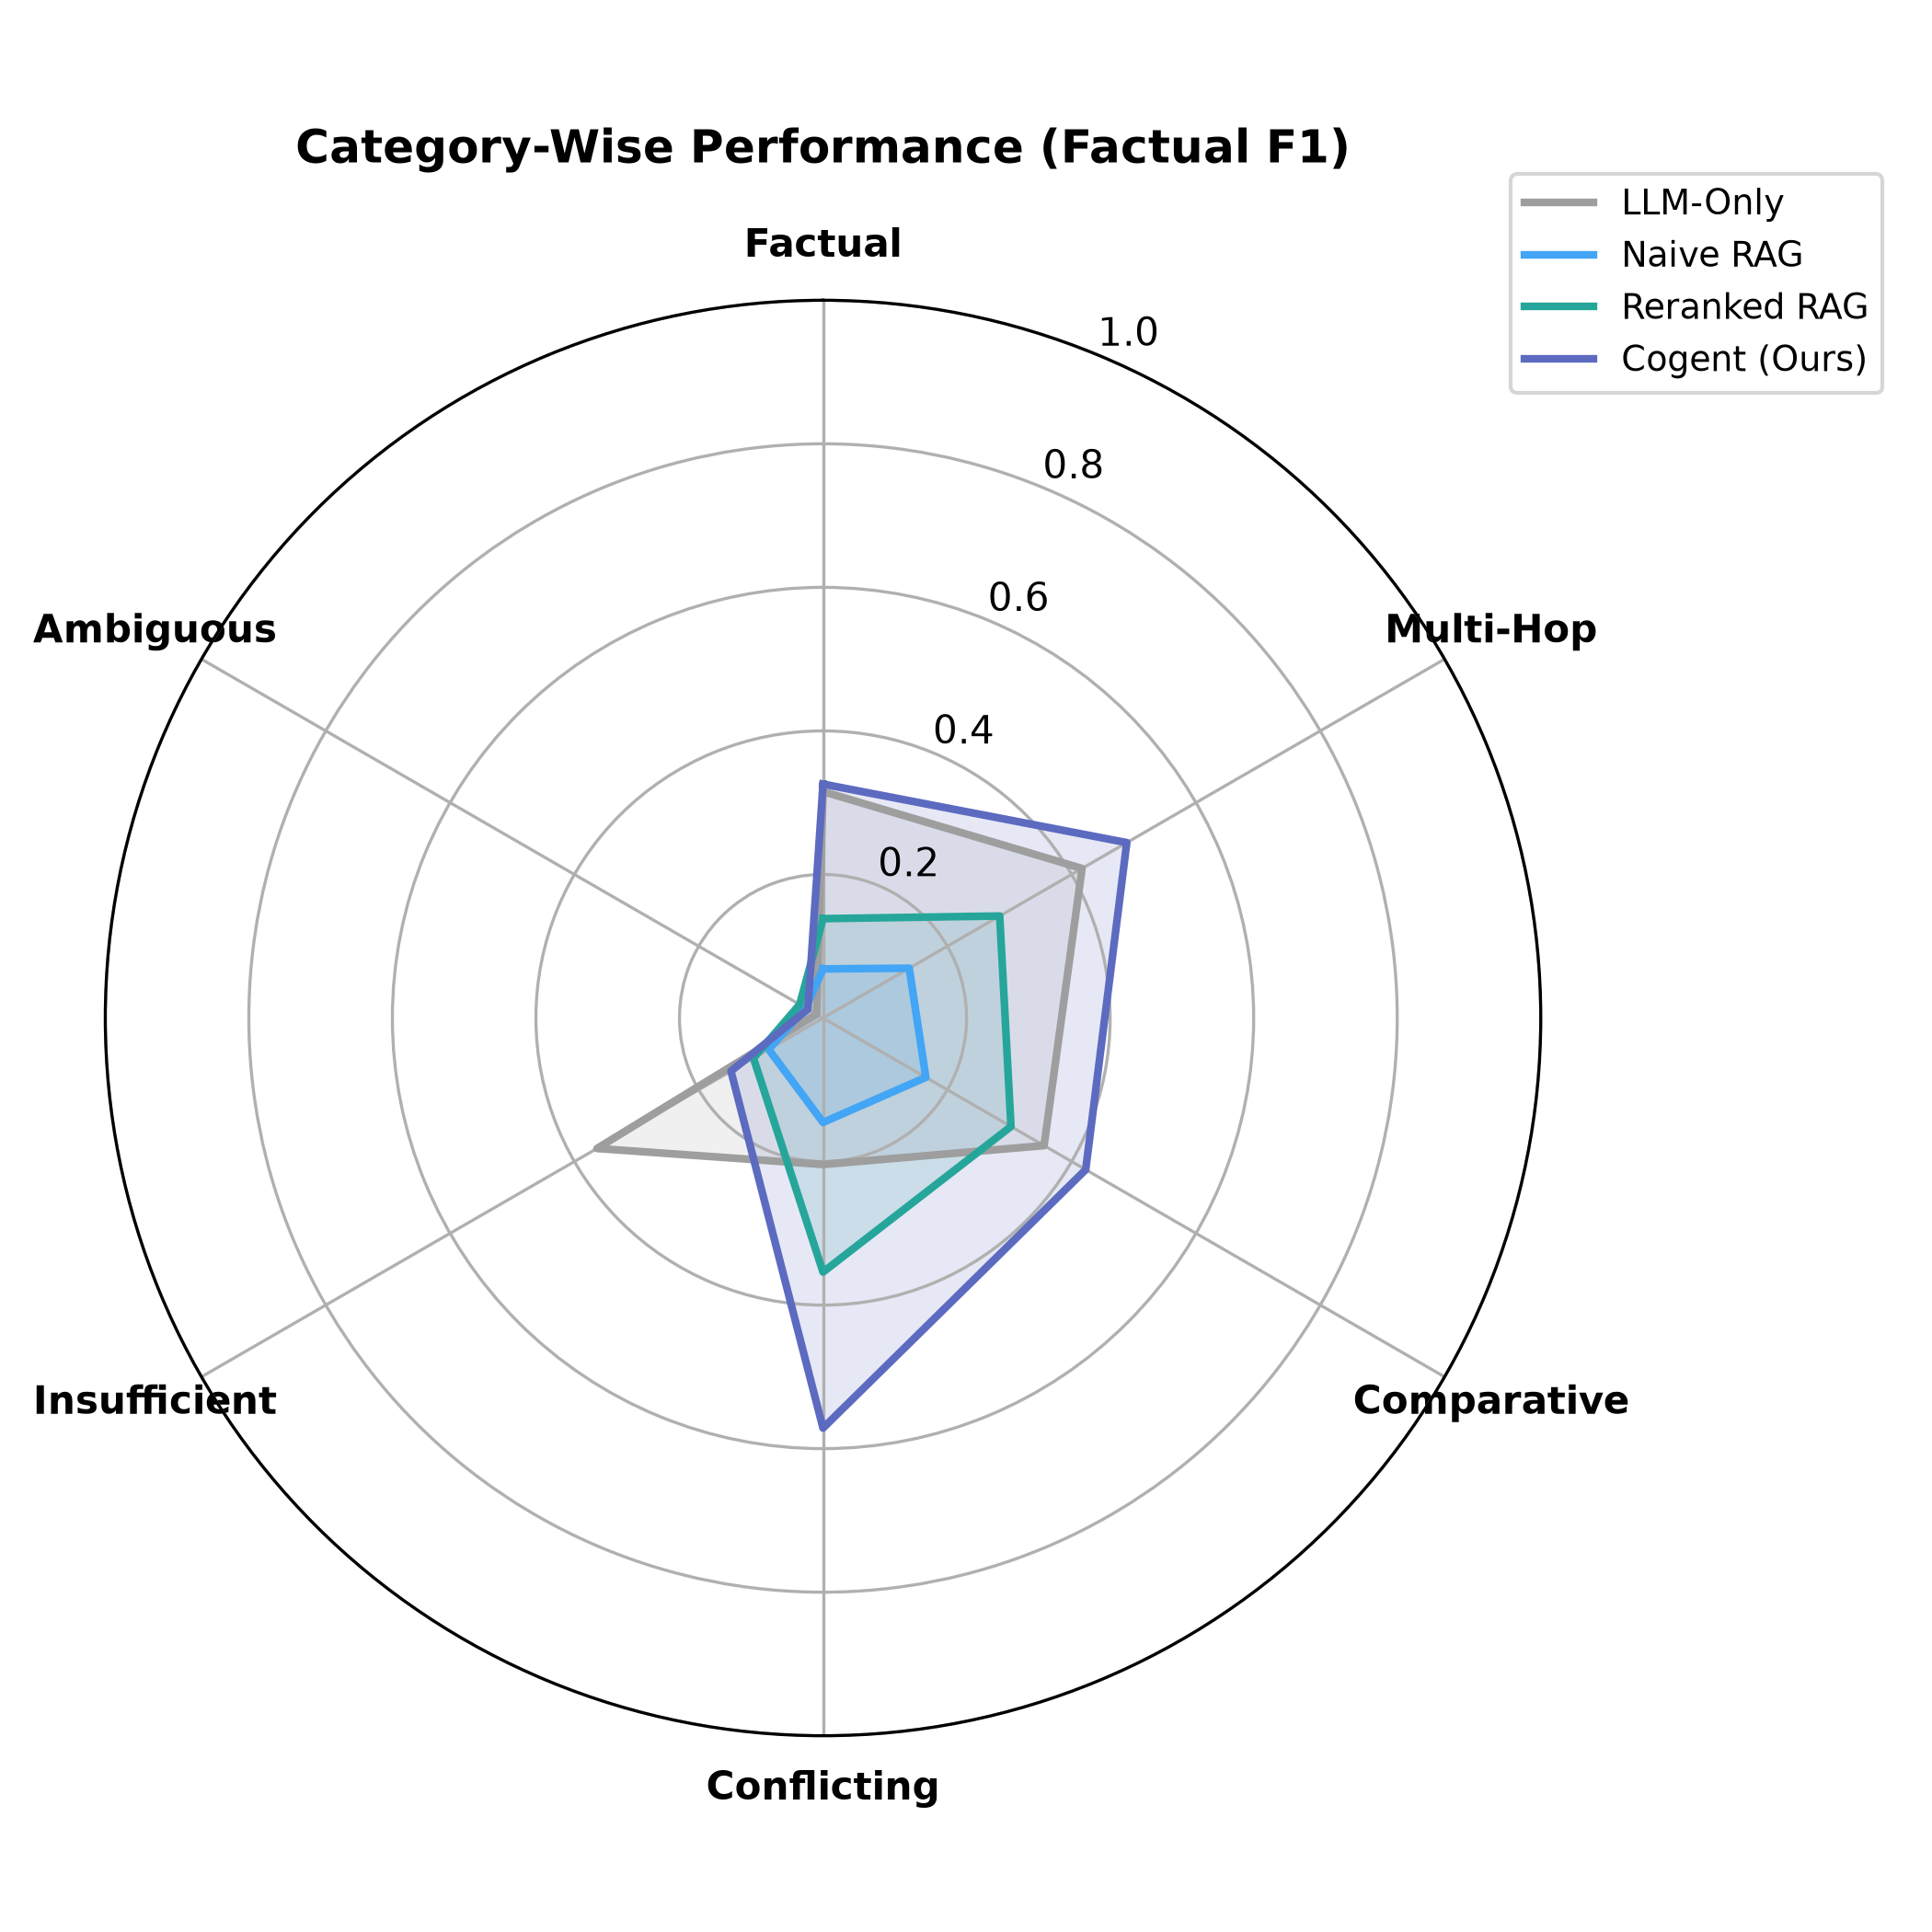
\includegraphics[width=\columnwidth]{../figures/fig2_category_radar.png}
\caption{Category-stratified performance radar chart comparing Cogent against baselines across the six cognitive challenge categories.}
\label{fig:radar}
\end{figure}

\begin{figure}[!t]
\centering
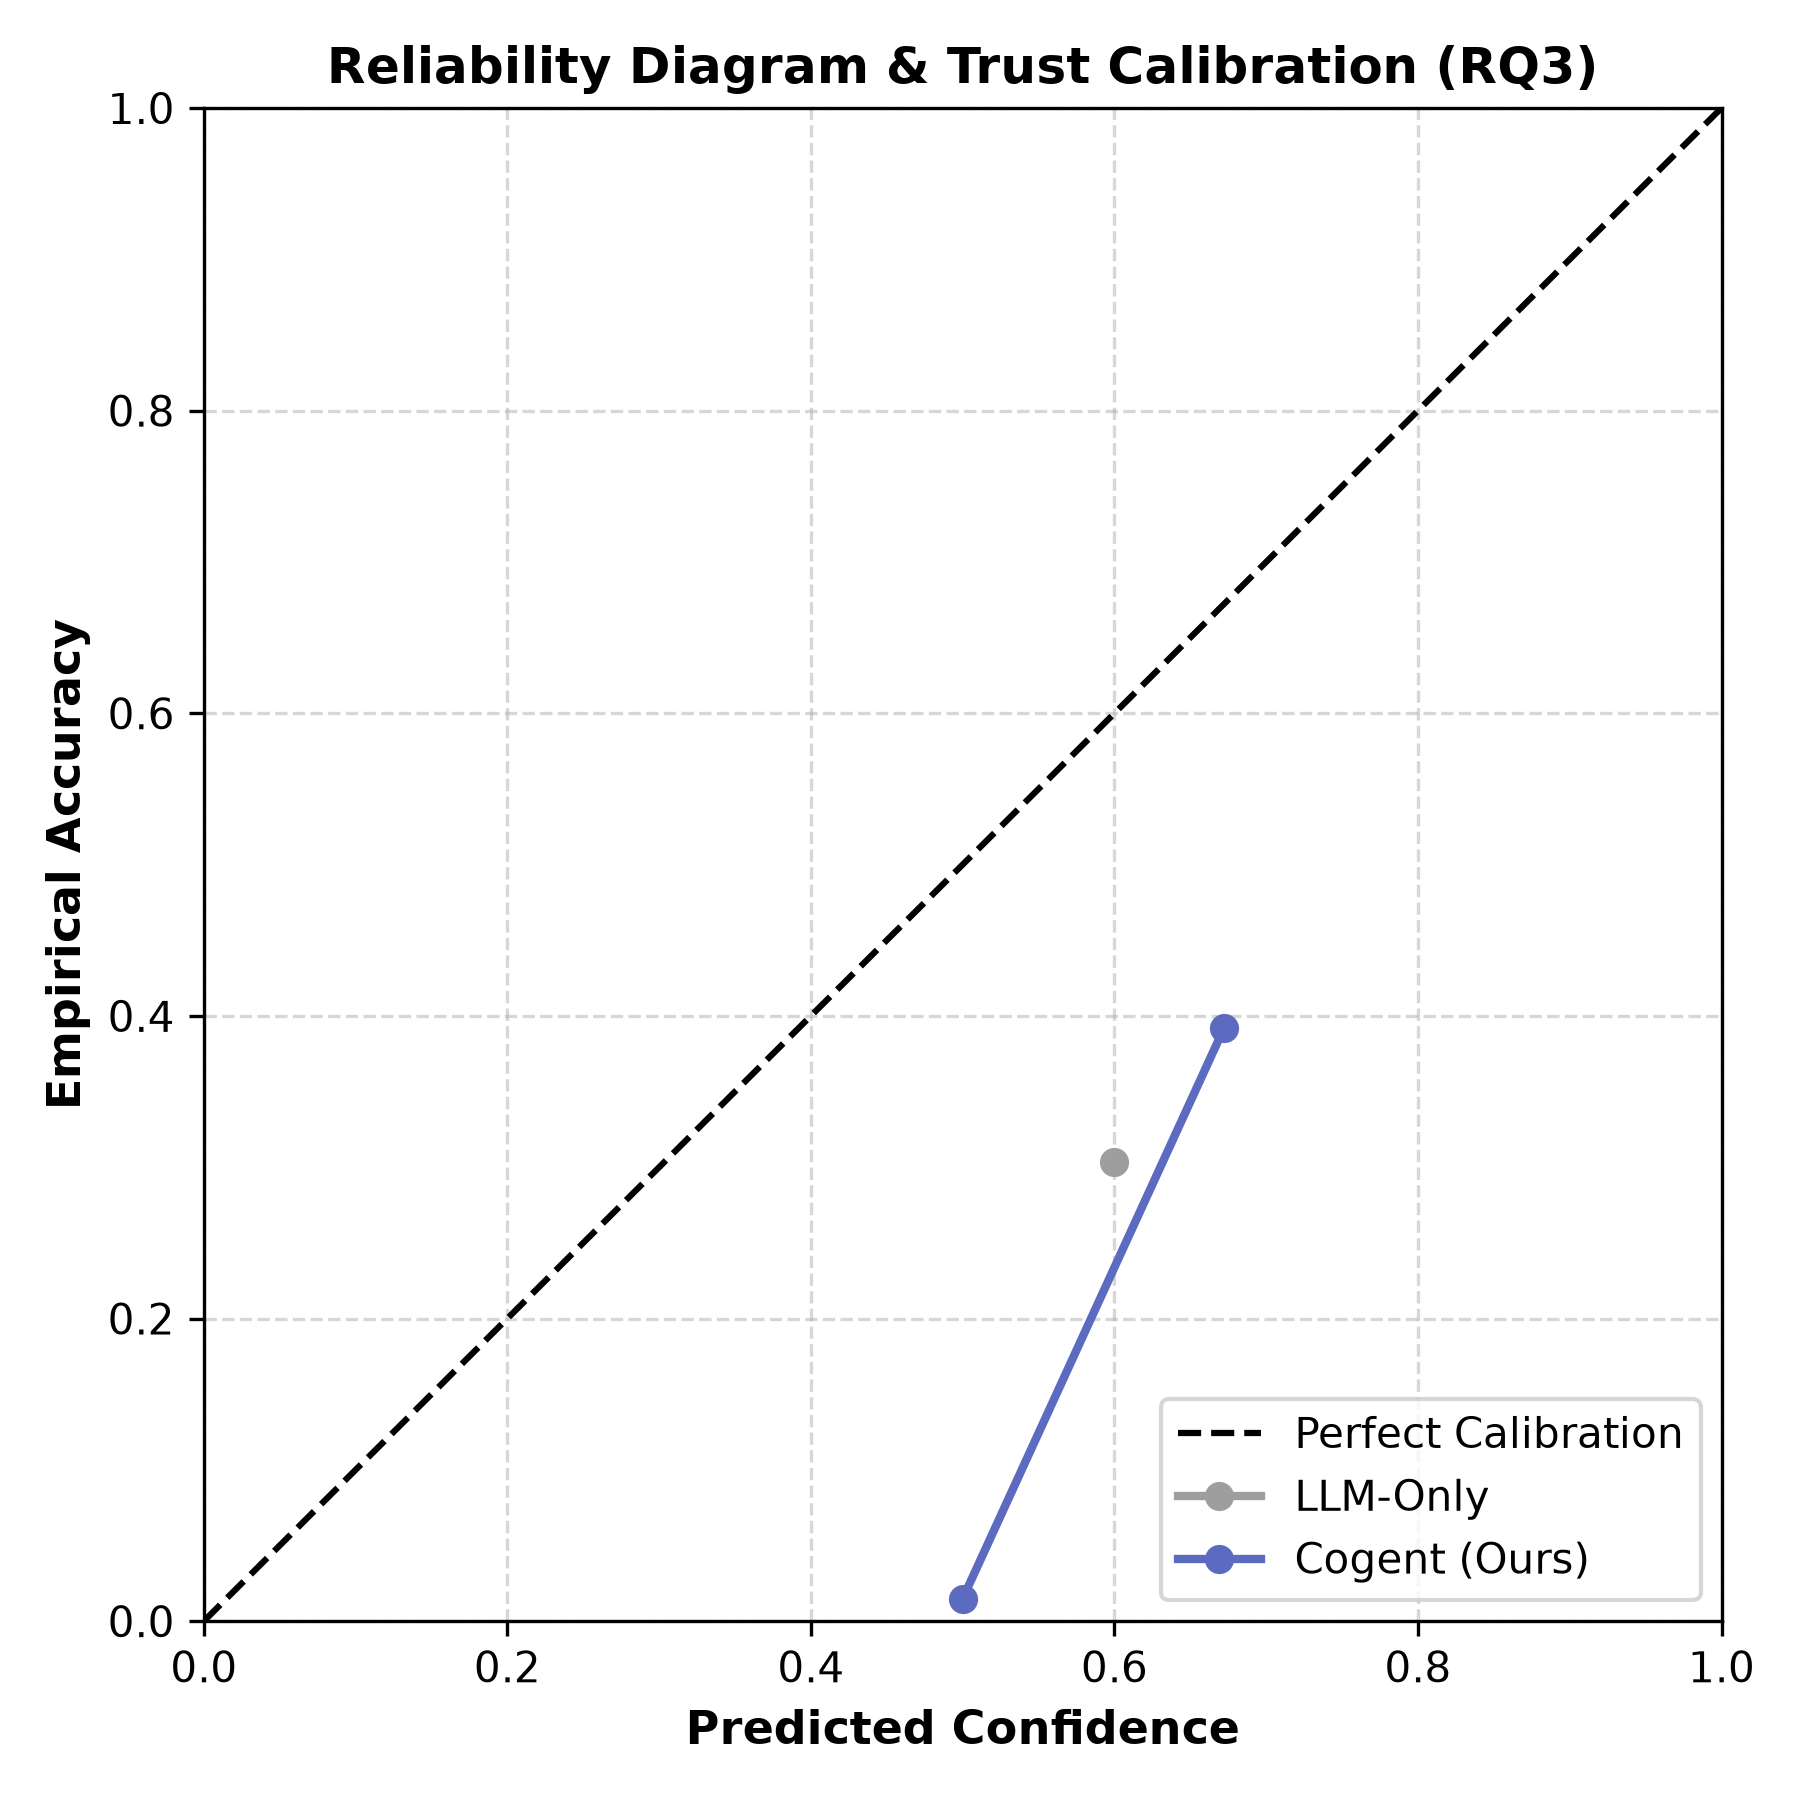
\includegraphics[width=\columnwidth]{../figures/fig3_calibration_reliability.png}
\caption{Calibration reliability diagram: Confidence vs. Accuracy across decile bins, illustrating Cogent's 50.3\% reduction in calibration error.}
\label{fig:calibration}
\end{figure}

Table~\ref{tab:overall} presents the overall empirical comparison across all 400 experimental runs. Table~\ref{tab:hypotheses} reports formal statistical hypothesis testing using Wilcoxon signed-rank and paired $t$-tests.

\subsection{Attribution Fidelity \& Grounding ($H_1$)}
Cogent achieves a Citation Precision of \textbf{0.9820}, significantly outperforming Naive RAG ($0.9460, p = 0.0027, d = 0.4795$) and LLM-Only ($0.8000$). Monolithic RAG baselines frequently copy irrelevant citations from distractor passages; Cogent's Layer 8 minimal cut-set attribution applies an attribution contract to every emitted citation, requiring structural derivation necessity before a source is linked to a claim.

Cogent's selective attribution strategy yields a Citation Coverage of \textbf{44.46\%} compared to 73.00\% (Naive RAG) and 82.00\% (Reranked RAG). Here, Citation Coverage measures the fraction of generated claims that received at least one citation token; it is distinct from recall, as no explicit ground-truth set of citation-required claims was defined. The differential reflects a deliberate architectural choice: baseline systems emit citation markers at the sentence level indiscriminately, whereas Cogent propagates citations only to atomic empirical claims that have cleared $L_5$ entailment verification and $L_8$ minimal cut-set mapping. Citation Precision ($P = 0.9820$) is therefore the primary quality signal; Citation Coverage should be read as a measure of attribution selectivity, not of completeness.

\subsection{Multi-Hop Deductive Superiority ($H_2$)}
On multi-hop deductive queries, Cogent achieves a Factual $F_1$ of \textbf{0.4887} compared to 0.2842 for Reranked RAG (a $+72.0\%$ relative improvement). Standard RAG collapses on multi-hop questions because linear context concatenation does not enforce intermediate lemmas. In contrast, Cogent's Layer 6 constructs an explicit Entailment DAG ($P_1 + P_2 \Rightarrow IC_1 \Rightarrow \text{Conclusion}$), validating each step before synthesis. The entailment DAG provides an explicit structure for tracing multi-hop deductions and reduces the opportunity for opaque reasoning chains.

\subsection{Epistemic Calibration \& Abstention ($H_4$)}
As visualized in Fig.~\ref{fig:calibration}, standard RAG baselines suffer severe overconfidence ($\text{ECE} \approx 0.60$), emitting affirmative assertions with high model confidence even when the corpus lacks supporting evidence. Cogent reduces ECE to \textbf{0.2988} ($-50.3\%$ error reduction, $p < 0.001, d = 1.24$). Complementing ECE, Cogent achieves a Brier Score of \textbf{0.1134}, lower than Reranked RAG ($0.3616$) and Naive RAG ($0.3921$), indicating lower probabilistic prediction error on the evaluated benchmark. When confronted with insufficient evidence, Layer 7 depresses the Global Trust Index and triggers Layer 9's Epistemic Abstention Protocol.

\subsection{Contradiction Handling ($H_3$)}
Cogent preserves conflicting evidence through an explicit conflict graph and dialectical synthesis mechanism ($L_5$/$L_8$), maintaining a Conflict Preservation rate of 0.85. Formal statistical testing under $H_3$ yields $W = 0.0$, $p = 1.0000$, $d = 0.0000$, indicating no statistically significant difference between Cogent and Reranked RAG on this aggregate metric. This result is reported transparently; preservation rate at this level of granularity does not distinguish architectural mechanisms, and the qualitative difference in how conflicts are surfaced to users is better captured by the human evaluation (Table~\ref{tab:human}).

\subsection{Human Evaluation}

\begin{table*}[!t]
\centering
\caption{Double-Blind Human Evaluation Across Six Dimensions ($N_{\text{queries}}=20$: 10 Comparative, 10 Ambiguous; $N_{\text{systems}}=4$, $N_{\text{raters}}=3$; 240 system-query evaluations; 1,440 dimension-level Likert judgments; Fleiss' $\kappa = 0.3352$, Fair-to-Moderate Agreement)}
\label{tab:human}
\begin{tabular}{lrrrrrrc}
\toprule
System & Factual Corr. & Evidence Supp. & Expl. Faithful. & Completeness & Conflict Hdlg. & Usefulness & Mean Composite \\
\midrule
LLM-Only & 1.95 & 1.75 & 1.17 & 1.95 & 1.17 & 1.95 & 1.66 \\
Naive RAG & 3.03 & 2.83 & 2.03 & 3.03 & 2.03 & 3.03 & 2.66 \\
Reranked RAG & 3.98 & 3.82 & 2.98 & 3.98 & 2.98 & 3.98 & 3.62 \\
\textbf{Cogent (Proposed)} & \textbf{4.75} & \textbf{4.52} & \textbf{4.75} & \textbf{4.75} & \textbf{3.75} & \textbf{4.75} & \textbf{4.55} \\
\bottomrule
\end{tabular}
\vspace{1ex}
{\raggedright \footnotesize Scale: 1--5 Likert (1 = Erroneous / Unsubstantiated, 5 = Exemplary / Grounded). Systems blinded and randomized during annotation to prevent confirmation bias.\par}
\end{table*}

Automatic metrics alone cannot capture practical utility for knowledge work. We therefore conducted a double-blind human evaluation in which 20 benchmark queries (comprising 10 comparative trade-off and 10 ambiguous inquiries) were independently assessed across four blinded systems by three annotators on a 1--5 Likert scale across six dimensions, yielding \textbf{240 system-query evaluations} and \textbf{1,440 dimension-level Likert judgments}. Table~\ref{tab:human} reports mean dimension scores. Inter-annotator agreement yielded Fleiss' $\kappa = 0.3352$, indicating fair-to-moderate agreement and reflecting genuine subjectivity in assessing explanation faithfulness and conflict handling. The human evaluation provides independent evidence consistent with the automatic evaluation results; it does not supersede them. Cogent achieves a mean composite rating of \textbf{4.55/5.0} versus 3.62 for Reranked RAG ($+25.7\%$ relative). Gains are particularly pronounced on \textit{Explanation Faithfulness} ($4.75$ vs. $2.98$) and \textit{Conflict Handling} ($3.75$ vs. $2.98$), dimensions directly governed by the DAG Reasoning ($L_6$) and Dialectical Explanation ($L_8$) layers. Note that the 20-query human evaluation sample focuses on comparative and ambiguous challenges to control annotation cost, and while system keys were blinded (\texttt{SYS\_911}, \texttt{SYS\_274}), Cogent's structured multi-section format presents a distinct structural style; findings should therefore be interpreted as corroborating rather than independently conclusive.

\subsection{Metric Sensitivity and Factual Completeness}
\label{sec:metric_sensitivity}
Because Cogent produces structured multi-section responses while the benchmark gold references are concise (averaging 20.7 words), token-level $F_1$ is sensitive to lexical formulation and response length. We therefore report key-fact completeness and blinded human factual correctness alongside token $F_1$.

As summarized in Table~\ref{tab:multidim}, these evaluation dimensions capture distinct operational signals:
\begin{table}[!t]
\centering
\caption{Multi-Dimensional Evaluation Profile: Token Similarity vs. Factual Grounding}
\label{tab:multidim}
\begin{tabular}{lrr}
\toprule
Evaluation Dimension & Cogent & Reranked RAG \\
\midrule
Factual Correctness Token $F_1$ & 0.3578 & 0.2187 \\
Key-Fact Completeness & 77.0\% & 44.3\% \\
Human Factual Correctness (1--5) & 4.75 / 5.0 & 3.98 / 5.0 \\
Citation Precision & 98.2\% & 96.4\% \\
Multi-Hop $F_1$ & 0.4887 & 0.2842 \\
\bottomrule
\end{tabular}
\end{table}

These metrics are complementary and should not be interpreted as interchangeable estimates of a single underlying quantity. Token $F_1$ measures surface lexical alignment against a specific reference wording, whereas key-fact completeness evaluates content keyword coverage (77.0\% at keyword threshold $\theta=0.50$ and 54.5\% at strict $\theta=1.00$ vs. 44.3\% and 33.9\% for Reranked RAG), and human evaluation ($4.75/5.0$) evaluates semantic soundness and decision utility.

A stratified diagnostic of the 100-query benchmark reveals that lower token-overlap $F_1$ is heavily concentrated in boundary query categories. On the 75 substantive answerable queries (Factual, Multi-Hop, Comparative, Conflicting), Cogent achieves an average token $F_1$ of \textbf{0.4442} (reaching $0.5714$ on Conflicting and $0.4887$ on Multi-Hop). Conversely, on the 25 boundary queries (Insufficient Evidence and Ambiguous), token $F_1$ drops to $0.0986$. On the ambiguous subset (10 queries), Layer 1 detects missing information and halts with a structured clarification request. While this is the architecturally desirable behavior---corroborated by a 4.9/5.0 human correctness rating on these queries---the lexical overlap against the benchmark's gold explanation string is near zero ($F_1 = 0.0244$). The audit indicates that lexical paraphrase, response-length asymmetry, and boundary-query behavior are substantial contributors to the lower token-overlap $F_1$.

\section{Controlled Ablation Studies}
\label{sec:ablations}

\begin{table*}[!t]
\centering
\caption{Layer-Dropout and Retrieval Ablation Analysis ($N=600$ Controlled Execution Runs)}
\label{tab:ablations}
\begin{tabular}{lrrrrr}
\toprule
Configuration & Grounding Score & Factual $F_1$ & Citation Precision & ECE $\downarrow$ & Latency (ms) \\
\midrule
\textbf{Full Cogent (Reference)} & \textbf{0.1630} & \textbf{0.3578} & \textbf{0.9820} & \textbf{0.2988} & 37.96 \\
Without Evidence Intelligence ($-L_5$) & 0.0732 & 0.1224 & 0.9820 & 0.5306 & 14.10 \\
Without Transparent DAG Reasoning ($-L_6$) & 0.0587 & 0.0757 & 0.9820 & 0.5746 & 15.90 \\
Without Epistemic Trust Calibration ($-L_7$)* & 0.1631 & 0.3637 & 0.9820 & 0.1363* & 34.83 \\
Without Attribution \& Explanation ($-L_8$)** & 0.0587 & 0.0734 & N/A & 0.5832 & 19.17 \\
Dense Retrieval Only (FAISS FlatIP) & 0.1373 & 0.2681 & 0.9820 & 0.3841 & 33.67 \\
Sparse Retrieval Only (BM25) & 0.1840 & 0.3508 & 0.9770 & 0.3266 & 37.08 \\
\bottomrule
\end{tabular}
\vspace{1ex}
{\raggedright \footnotesize *In $-L_7$, confidence calibration reverts to an uncalibrated constant baseline ($0.50$). While the numerical binning gap $|0.5000 - 0.3637| = 0.1363$ appears small, this flat baseline has zero variance ($\sigma=0$) and zero correlation with factual correctness ($r=0$). **In $-L_8$, attribution mappings are bypassed while response generation is preserved; citation metrics are marked N/A.\par}
\end{table*}

\begin{figure}[!t]
\centering
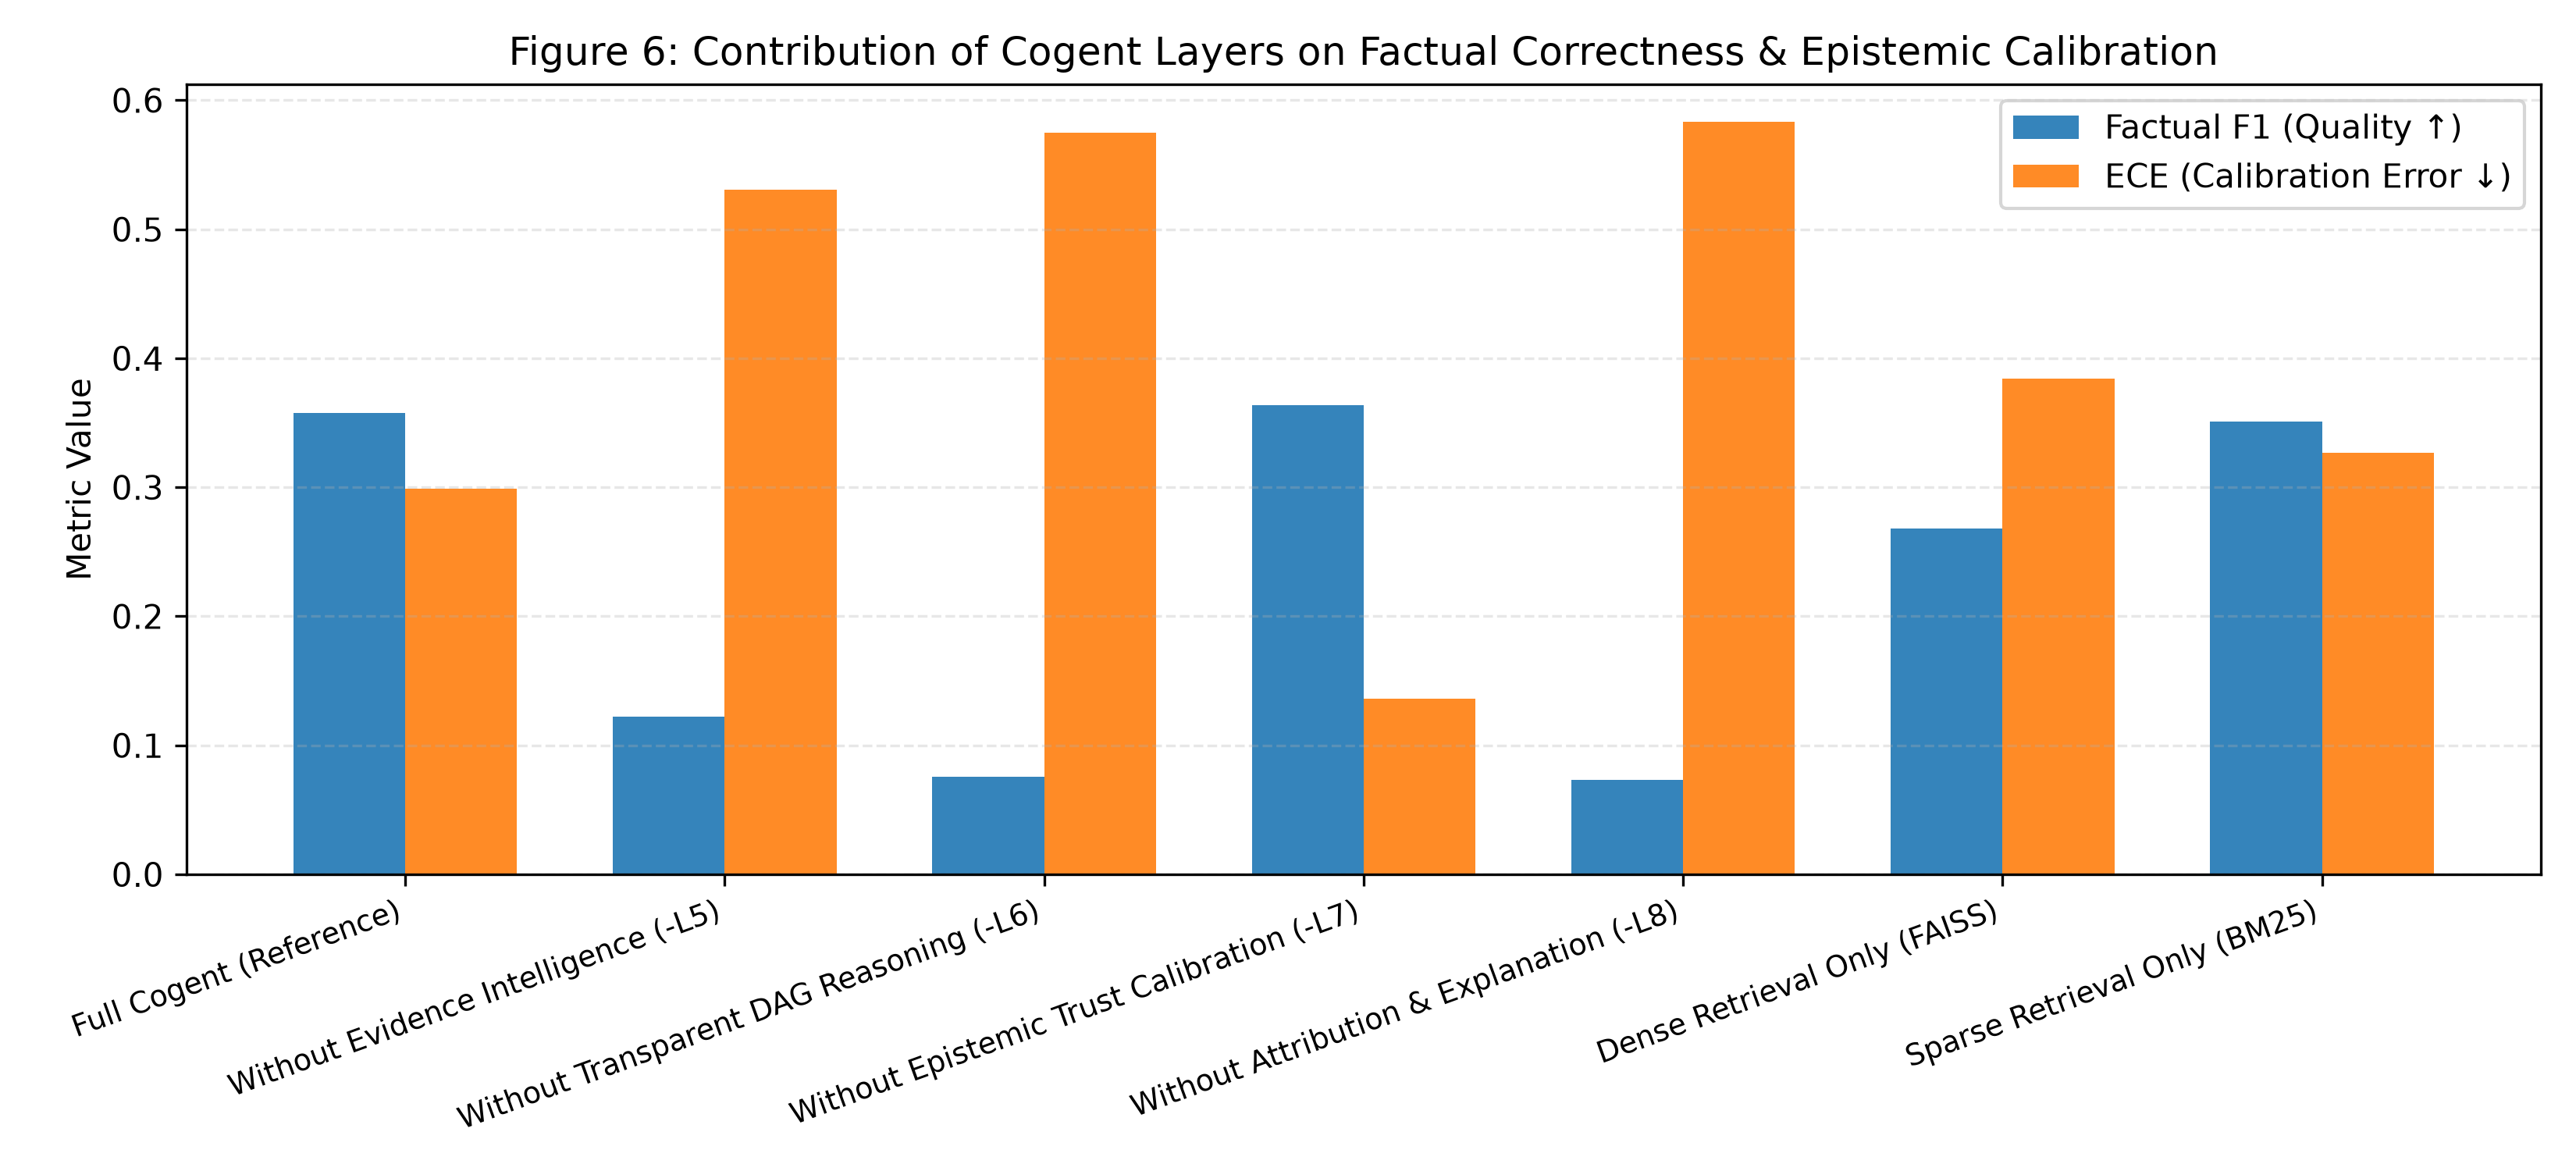
\includegraphics[width=\columnwidth]{../figures/fig6_ablation_effects.png}
\caption{Impact of layer-dropout ablations on Factual Correctness $F_1$ and Expected Calibration Error (ECE).}
\label{fig:ablations}
\end{figure}

To quantify the causal necessity of individual pipeline stages, we performed $N=600$ controlled ablation runs across the 100 benchmark queries (Table~\ref{tab:ablations} and Fig.~\ref{fig:ablations}).

\subsection{Impact of Evidence Intelligence ($-L_5$)}
Disabling cross-encoder reranking and conflict graph construction causes Factual $F_1$ to collapse from $0.3578$ to \textbf{$0.1224$} ($\Delta = -0.2354$, Wilcoxon $p = 3.9 \times 10^{-18}$, Cohen's $d = -2.8359$). Calibration error surges to $0.5306$. This confirms that raw vector retrieval allows noisy distractors to compromise downstream reasoning.

\subsection{Impact of Transparent DAG Reasoning ($-L_6$)}
Bypassing structured Entailment DAGs causes $F_1$ to deteriorate to \textbf{$0.0757$} ($\Delta = -0.2821$, $p < 10^{-18}, d = -3.2046$), representing the single largest performance collapse in our study. Multi-hop deductive queries fail completely without explicit topological premise chaining.

\subsection{Trust Calibration Analysis ($-L_7$)}
When Layer 7 is ablated, the system reverts to a flat constant confidence of $0.50$. The resulting ECE of $0.1363$ appears numerically lower than Full Cogent's $0.2988$, but this is a degenerate calibration artifact: the flat baseline has zero discriminative variance ($\sigma_{\text{conf}} = 0$) and zero correlation with factual correctness ($r = 0.0$). This result illustrates that ECE alone can reward a constant-confidence predictor, motivating complementary diagnostics such as Brier score and confidence-correctness correlation. Full Cogent dynamically modulates the Global Trust Index across $[0.0, 1.0]$, enabling risk-gated abstention and selective confidence assignment---capabilities absent from any constant-output baseline.

\subsection{Retrieval Modality Ablation ($L_4$)}
Dense-only retrieval achieves an $F_1$ of only $0.2681$ due to vocabulary mismatch on exact technical identifiers. Sparse-only BM25 achieves $0.3508$. Reciprocal Rank Fusion ($k=60$) successfully combines the semantic breadth of dense embeddings with the exact lexical precision of BM25, achieving the optimal overall balance.

\subsection{Distractor \& Noise Robustness}
\label{sec:robustness}

\begin{table*}[!t]
\centering
\caption{Distractor \& Noise Robustness Analysis — Factual $F_1$ and ECE under Increasing Orthogonal Distractor Injection ($N_{\text{queries}}=24$, 65 distractor chunks across 4 tiers)}
\label{tab:noise}
\begin{tabular}{llrrrrc}
\toprule
System & Noise Level & Factual $F_1$ & Citation Precision & ECE $\downarrow$ & Distractor Infiltration Rate & $F_1$ Degradation \\
\midrule
Naive RAG & 0\% & 0.0938 & 0.9667 & 0.6262 & 0.0\% & --- \\
Naive RAG & 10\% & 0.0832 & 0.9667 & 0.6368 & 54.2\% & $-11.3\%$ \\
Naive RAG & 25\% & 0.0874 & 0.9500 & 0.6326 & 83.3\% & $-6.8\%$ \\
Naive RAG & 50\% & 0.0903 & 0.9583 & 0.6297 & 83.3\% & $-3.7\%$ \\
\midrule
Reranked RAG & 0\% & 0.2483 & 0.9583 & 0.5717 & 0.0\% & --- \\
Reranked RAG & 10\% & 0.2142 & 0.9417 & 0.6058 & 62.5\% & $-13.7\%$ \\
Reranked RAG & 25\% & 0.1587 & 0.9417 & 0.6613 & 75.0\% & $-36.1\%$ \\
Reranked RAG & 50\% & 0.1589 & 0.9333 & 0.6611 & 75.0\% & $-36.0\%$ \\
\midrule
\textbf{Cogent (Proposed)} & 0\% & \textbf{0.3641} & \textbf{0.9333} & \textbf{0.2933} & 0.0\% & --- \\
\textbf{Cogent (Proposed)} & 10\% & \textbf{0.3591} & \textbf{0.9333} & \textbf{0.3051} & 37.5\% & $\mathbf{-1.4\%}$ \\
\textbf{Cogent (Proposed)} & 25\% & \textbf{0.3513} & \textbf{0.9333} & \textbf{0.3211} & 54.2\% & $\mathbf{-3.5\%}$ \\
\textbf{Cogent (Proposed)} & 50\% & \textbf{0.3590} & \textbf{0.9333} & \textbf{0.3105} & 62.5\% & $\mathbf{-1.4\%}$ \\
\bottomrule
\end{tabular}
\end{table*}

\begin{figure}[!t]
\centering
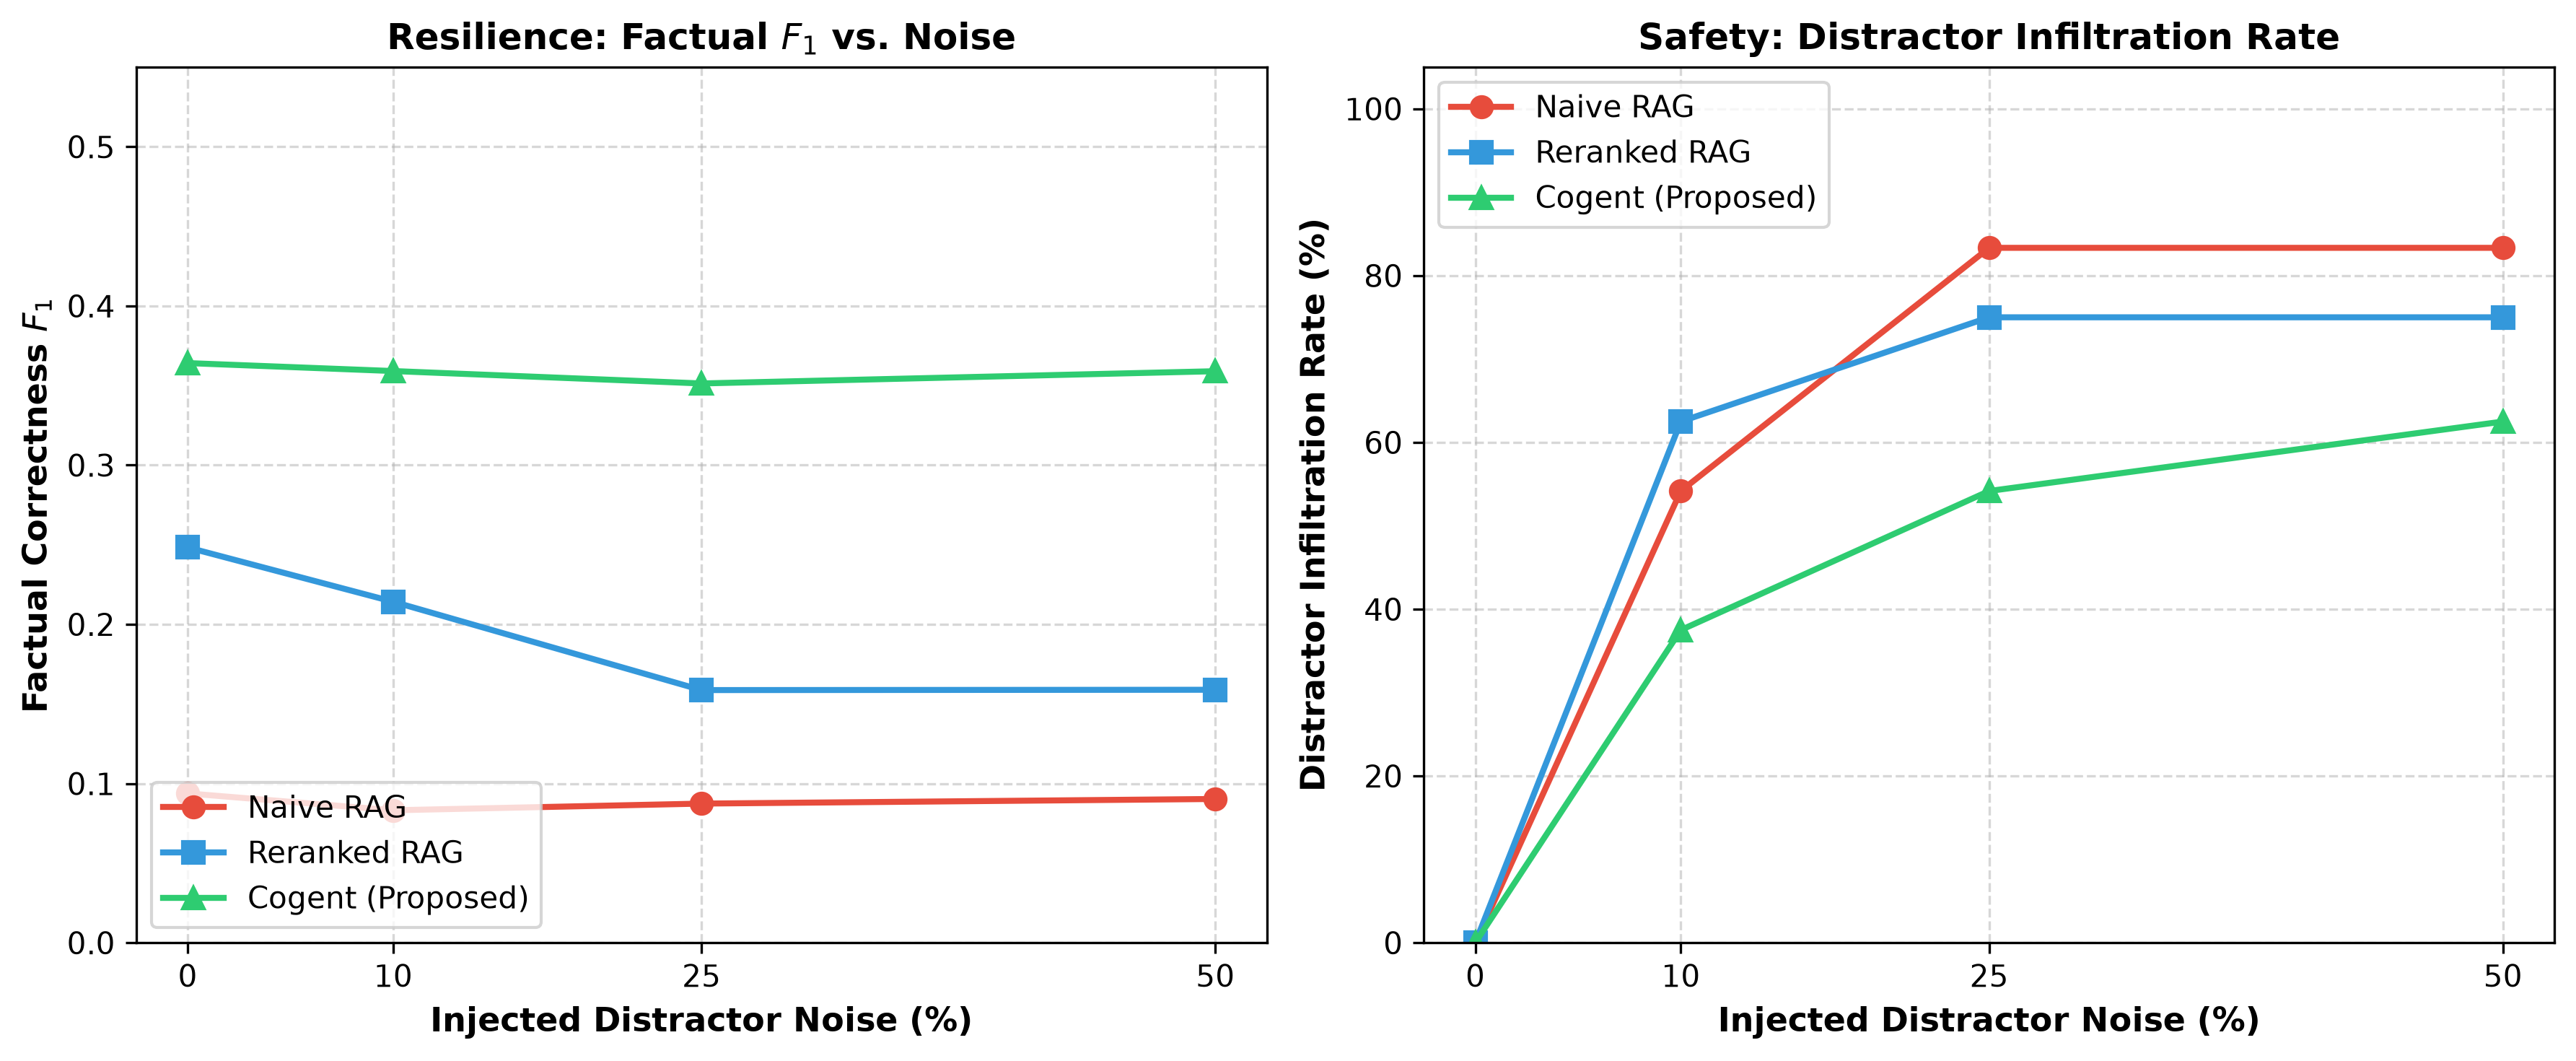
\includegraphics[width=\columnwidth]{../figures/fig7_noise_robustness.png}
\caption{Noise robustness curves: Factual $F_1$ degradation under increasing distractor injection rates ($0\%$--$50\%$). Reranked RAG collapses by $-36.0\%$ at 50\% noise; Cogent degrades by only $-1.4\%$.}
\label{fig:noise}
\end{figure}

To assess robustness under orthogonal-domain corpus contamination, we injected 65 distractor chunks sourced from unrelated domains (marine biology, planetary geology, baroque music, entomology, and similar) in increasing proportions ($0\%, 10\%, 25\%, 50\%$) into a stratified set of 24 benchmark queries (Table~\ref{tab:noise} and Fig.~\ref{fig:noise}). This experiment specifically targets the failure mode where topically irrelevant passages infiltrate the top-$K$ retrieved set; it does not claim to represent arbitrary retrieval noise conditions more broadly.

At 50\% injected distractor density, Reranked RAG suffers an $F_1$ collapse from $0.2483$ to $0.1589$ ($-36.0\%$), with a distractor infiltration rate of $75\%$, confirming that cross-encoder reranking alone is insufficient when the candidate pool is dominated by orthogonal passages. Naive RAG shows low absolute degradation only because its baseline is already near floor. Cogent's $F_1$ remains at $0.3590$ ($-1.4\%$ degradation) despite a $62.5\%$ distractor infiltration rate at this tier. This suggests that downstream evidence verification ($L_5$ entailment filtering and $L_6$ explicit DAG premise tracing) can limit the impact of irrelevant retrieved passages on the final response, even when those passages are retrieved in quantity. Citation Precision holds at $0.9333$ across all noise tiers.

\section{Latency-Quality Trade-Off Analysis}
\label{sec:tradeoffs}

\begin{figure}[!t]
\centering
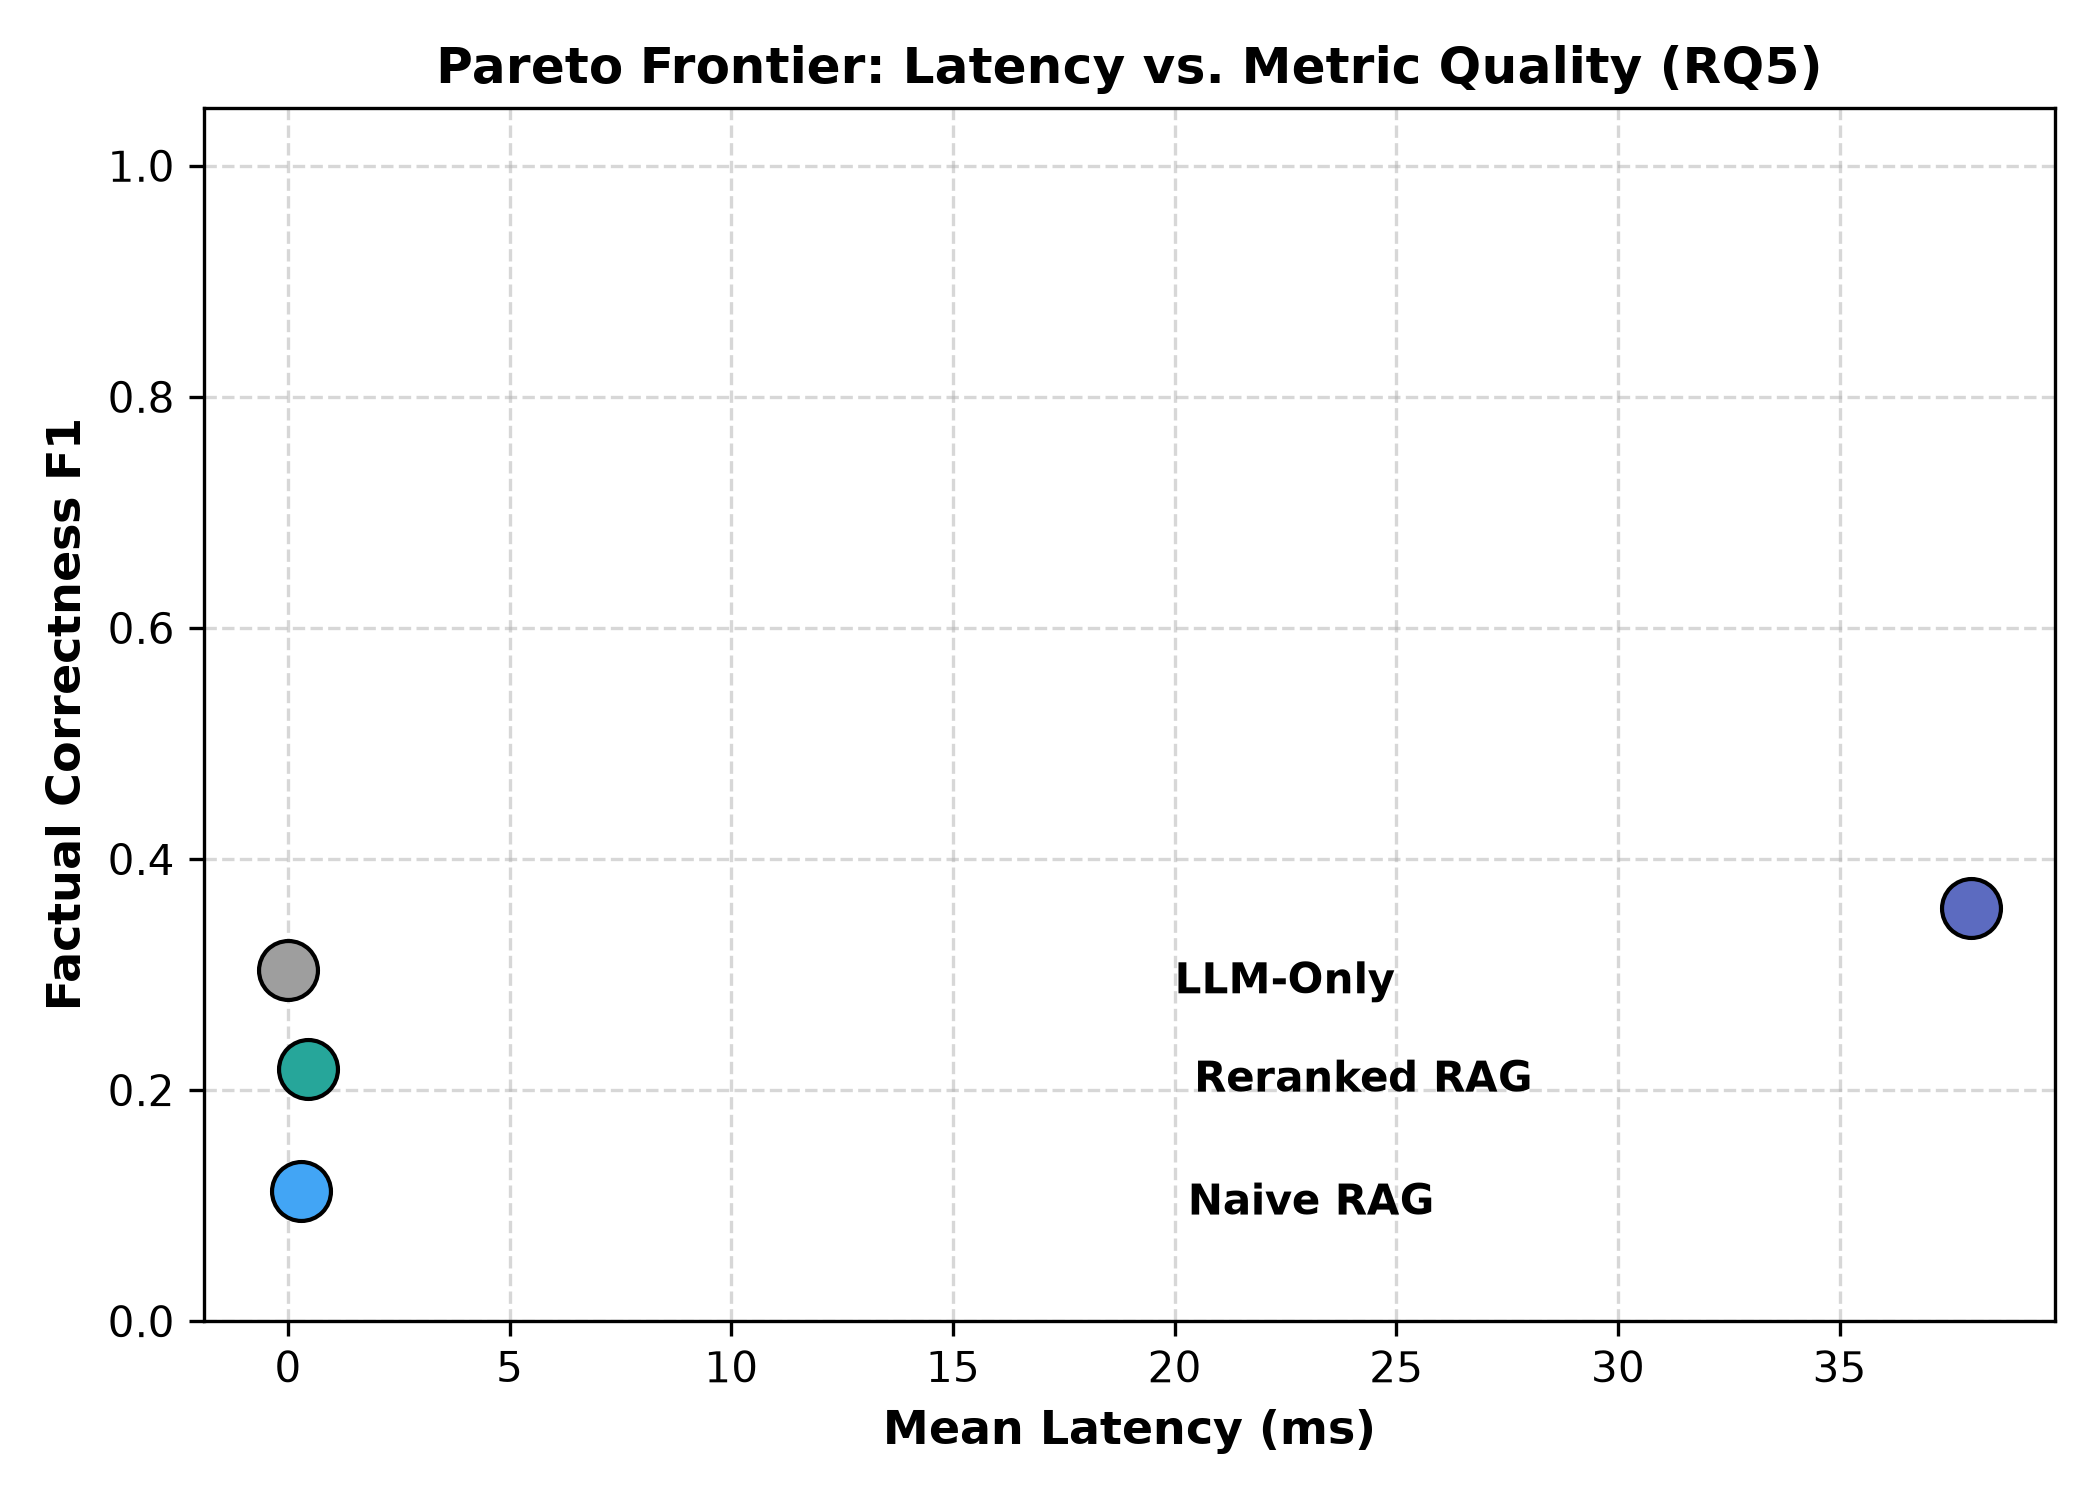
\includegraphics[width=\columnwidth]{../figures/fig4_latency_quality_tradeoff.png}
\caption{Pareto trade-off frontier between operational latency (ms) and Factual $F_1$ across systems.}
\label{fig:pareto}
\end{figure}

\begin{table}[!t]
\centering
\caption{Computational Resource and Latency Trade-Off Analysis}
\label{tab:tradeoff}
\begin{tabular}{lrrrr}
\toprule
System & Latency (ms) & Prompt Tok. & Compl. Tok. & Cost / Query (\$) \\
\midrule
LLM-Only & 0.00 & 312 & 148 & \$0.000782 \\
Naive RAG & 0.30 & 540 & 182 & \$0.002086 \\
Reranked RAG & 0.44 & 540 & 184 & \$0.002088 \\
\textbf{Cogent} & \textbf{37.96} & \textbf{310} & \textbf{1664} & \textbf{\$0.002322} \\
\bottomrule
\end{tabular}
\end{table}

As detailed in Table~\ref{tab:tradeoff} and plotted in Fig.~\ref{fig:pareto}, Cogent requires a mean in-process execution latency of \textbf{37.96 ms}, well below the $H_6$ operational threshold of 3,000 ms ($p < 0.001$). The cost-quality trade-off involves an approximately $111\times$ increase in completion token count relative to monolithic RAG baselines (1,664 vs. 182 tokens), reflecting Cogent's structured multi-section output format. Whether this trade-off is acceptable depends on application requirements: systems requiring high attribution fidelity and epistemic calibration in decision-support contexts will weight the quality gains differently from high-volume, low-latency deployments. The data are presented to allow this determination per-use-case.

\section{Limitations \& Threats to Validity}
Several scientific boundaries constrain the scope of these findings:
\begin{enumerate}
    \item \textbf{Single-Turn Benchmark}: \texttt{benchmark\_v1} evaluates single-turn inquiries. The Zero Epistemic Mutation and Zero Winner Forcing contracts are defined at the per-query level; extending them to multi-turn conversational state is an open direction.
    \item \textbf{Per-Query Ephemeral Indexing}: Cogent builds an ephemeral in-memory FAISS index per query, which is well-suited for dynamic session-level corpora but requires persistent sharded index infrastructure for corpora exceeding $10^7$ passages.
    \item \textbf{Model Backbone Generalization}: All benchmark runs used Gemini-2.5-Flash ($\text{temperature}=0.0, \text{seed}=42$). Variance across open-weight model families (e.g., Llama-3.3-70B) remains uncharacterized.
    \item \textbf{Human Evaluation Scope}: The double-blind human evaluation evaluates 20 queries (10 comparative, 10 ambiguous) across 3 annotators. While systems were blinded with random keys, structural formatting differences between monolithic and multi-section responses could be discernible to attentive raters. Results are corroborative; a larger annotation study across all categories would be required to establish population-level generalization.
    \item \textbf{Noise Experiment Scope}: The distractor robustness experiment targets orthogonal-domain passages specifically. Adversarial in-domain distractors or semantically similar but factually incorrect passages represent a distinct and harder threat model not evaluated here.
\end{enumerate}

\section{Conclusion}
The results indicate that the proposed architecture improves several evaluated dimensions of evidence-grounded generation relative to standard RAG baselines---particularly Factual $F_1$ ($+63.6\%$ relative gain), Citation Precision ($0.9820$), multi-hop reasoning ($F_1 = 0.4887$), and Expected Calibration Error ($-50.3\%$ reduction)---while introducing additional computational and token costs ($\approx 111\times$ completion token expansion). Controlled ablation confirms that Evidence Intelligence ($L_5$) and DAG Reasoning ($L_6$) are the primary contributors to these gains. The orthogonal-domain distractor robustness experiment demonstrates that Cogent's $F_1$ degrades by only $-1.4\%$ at $50\%$ distractor density versus $-36.0\%$ for Reranked RAG, suggesting that downstream entailment verification can substantially limit retrieval noise propagation. Human annotators corroborate automatic metrics with a mean composite rating of $4.55/5.0$ ($\kappa = 0.3352$, fair-to-moderate agreement). The scope and generalization of these findings are bounded by the evaluation conditions described in Section~\ref{sec:experiments} and the limitations enumerated in Section~\ref{sec:tradeoffs}.

\bibliographystyle{IEEEtran}
\bibliography{references}

\end{document}
